\documentclass[b5paper,12pt]{book}
\usepackage[utf8]{inputenc}
\usepackage{graphicx}
\usepackage{setspace}
\usepackage[]{geometry}
\usepackage{amsmath}
\graphicspath{ {resources/images} }
\usepackage{multirow}
\usepackage{makecell}

\usepackage[skip=10pt]{parskip}

\usepackage{listings}
\usepackage{color}


\definecolor{dkgreen}{rgb}{0,0.6,0}
\definecolor{gray}{rgb}{0.5,0.5,0.5}
\definecolor{pink}{rgb}{0.87,0.59,0.7}
\definecolor{mauve}{rgb}{0.58,0,0.82}

\lstset{frame=l,
	language=C++,
	aboveskip=3mm,
	belowskip=3mm,
	showstringspaces=false,
	columns=flexible,
	basicstyle={\small\ttfamily},
	numbers=none,
	numberstyle=\tiny\color{pink},
	keywordstyle=\color{blue},
	commentstyle=\color{dkgreen},
	stringstyle=\color{mauve},
	breaklines=true,
	breakatwhitespace=true,
	tabsize=3
}

%CASES FORMATTING
\renewcommand\theadfont{\bfseries}

\newenvironment{casebox2}{	
	\begin{tabular}{|l|l|}	
		\hline
		\thead{Entrada} & \thead{Salida} \\
		\hline
}{	
	\end{tabular}	
}

\newenvironment{casebox3}{
	\begin{tabular}{|l|l|l|}
		\hline		
		\thead{Entrada} & \thead{Salida}& \thead{Expliación} \\
		\hline
}{	
	\end{tabular}	
}


\newcommand{\scase}[2]{
\makecell[tl]{#1}&\makecell[tl]{#2} \\
\hline
}
\newcommand{\ecase}[3]{
\makecell[tl]{#1}&\makecell[tl]{#2}&\makecell[tl]{#3} \\
\hline
}
% LIMIT LIST FORMATTING
\newenvironment{plimits}{\begin{itemize}
	\setlength{\parskip}{0.75pt}			
}{
\end{itemize}
}
% LINK COMMANDS
\newcommand{\omegalink}[1]{\small{www.omegaup.com/arena/problem/#1}}
\newcommand{\codeforceslink}[2]{\small{www.codeforces.com/problemset/problem/#1/#2}}
\newcommand{\codeforces}{Fuente: codeforces.com}

% FORMAT COMMANDS

\newcommand{\problembreak}{
\vspace{-\baselineskip}
\hrulefill
\vspace{-\baselineskip}
}

\begin{document}

\author{Héctor Fernando Ricárdez Lara}
\title{Búsquedas}
\date{}


\frontmatter
\maketitle
\renewcommand{\contentsname}{Índice}
\tableofcontents

\mainmatter
\chapter*{Introducción}
\addcontentsline{toc}{chapter}{Introducción}
\markboth{Introducción}{Introducción}


Muchas veces en nuestra vida hemos tenido que buscar algo, una foto en nuestra galería del teléfono, una palabra en el diccionario, una carta dentro de un mazo, etc. Y probablemente, con la experiencia, hemos aprendido algunas intuiciones sobre como buscar cosas, en este libro trabajaremos un poco más en desarrollar esta intuición e ideas.

Igual que en la vida diaria buscamos muchas cosas, en la resolución de problemas nos la pasamos buscando cosas, ya sea: la respuesta, algún valor en un arreglo, la raíz cuadrada de un número, etc.

Es decir, en estos problemas tendremos una lista de objetos y trataremos de encontrar en la lista uno que cumpla alguna propiedad especifica. Es decir, queremos encontrar una respuesta dentro de una lista de candidatos.

Entonces, búsqueda es simplemente encontrar una respuesta dentro en una lista de posibles candidatos.


\chapter* {Búsqueda lineal}
\addcontentsline{toc}{chapter}{Búsqueda lineal}
\markboth{Búsqueda lineal}{Búsqueda lineal}
La búsqueda lineal es la más sencilla de las búsquedas que hay. ¿Qué es lo que harías si te pido que de una pila de exámenes encuentres el tuyo? Lo que probablemente hagas es una revisar uno por uno, checar de arriba hacia abajo hasta que encuentres el examen con tu nombre en él.

Básicamente, esta idea es la búsqueda lineal, ir revisando de uno por uno toda una lista de candidatos hasta encontrar al que estas buscando o hasta que hayas revisado todos los candidatos.

Entonces, los códigos de búsqueda lineal casi siempre tendrán la siguiente estructura:

\begin{lstlisting}
Itera por cada candidato {
	Si el candidato es lo que buscamos {
		Respuesta = candidato;
		Detener ciclo /* esto es opcional, depende si hay varios valores que queramos encontrar. */
	}
}	
\end{lstlisting}

Veamos cómo usar esta técnica para resolver un problema.

\section*{Ejemplo 1.1}
\addcontentsline{toc}{section}{Ejemplo 1.1}

\subsection*{Descripción}
Supongamos que queremos tenemos un arreglo \(A\) de enteros distintos y este tiene \(N\) elementos en él. Nosotros querremos hacer un código que imprima la posición del arreglo que valga \(K\). O si este valor no existe, que imprima \(-1\).

\subsection*{Límites}
\begin{plimits}
	\item \(1\leq N \leq 10^5\)
	\item \(1\leq K,A[i] \leq 10^9\)
\end{plimits}
\subsection*{Solución}

(Recuerda intentar el problema antes de leer la solución)

Lo que este problema nos pide en realidad es buscar dentro del arreglo por el índice del elemento \(K\).

Lo que haremos es revisar todas las posiciones del arreglo hasta encontrar aquella que valga \(K\), si no la encontramos imprimimos \(-1\).


\subsection*{Código}
\begin{lstlisting}
int A[100050];
int N, K;
int main () {	
	ios_base::sync_with_stdio(0); cin.tie(0);
	cin >> N;
	for (int  i=0; i <N; i++){ 
		cin >> A[i];
	}
	cin >> K;
	int respuesta = -1;
	for (int i =0; i < N; i++) {
		if (A[i]==K) {
			respuesta = i;
			break;
		}
	}
	cout << respuesta;
}
\end{lstlisting}


\subsection*{Complejidad}

Una pregunta que te has de hacer es: ¿cuál es la complejidad de esta técnica? Y la respuesta es sencilla, en el peor de los casos tenemos que revisar a todos los candidatos, digamos que la cantidad de ellos es iguala a \(N\), entonces la complejidad es \(O(N)\).

\section*{Ejemplo 1.2}
\addcontentsline{toc}{section}{Ejemplo 1.2}
Veamos otro problema para aprender búsqueda lineal. 

\subsection*{Descripción}

Carlos quiere armar una fiesta, y como le gusta ser un buen anfitrión compro \(N\) regalos para sus invitados.
Ahora, Carlos quiere darle la misma cantidad de regalos a cada uno de sus invitados sin que sobre ningún regalo no repartido. Como Carlos le gusta contar, ahora se pregunta: ¿Cuántas cantidades diferentes de invitados puede tener?
\subsection*{Entrada}
Un entero \(N\), indicando cuantos regalos compró Carlos.
\subsection*{Salida}
La cantidad de posibles números de invitados para la fiesta.
\subsection*{Casos ejemplo}
\begin{casebox2}
	\scase{12}{6}
	\scase{7}{1}
	\scase{4}{3}
\end{casebox2}
\subsection*{Límites}
\begin{plimits}
	\item \(1\leq N \leq 10^5\)
\end{plimits}

\subsection*{Solución}
Es fácil ver que el problema en realidad pregunta: ¿Cuántos divisores positivos tiene \(N\)?

(Nota: un divisor de \(N\) es un número que divide a \(N\) sin decimales).

Encontremos todos los divisores de \(N\). Estos se encontrarán entre \(1\) y \(N\), por lo que podemos iterar i por todo este rango revisando si \(i\) es divisor de \(N\).
\subsection*{Código}
\begin{lstlisting}
respuesta = 0;
for (int i =1; i <= N; i++) {
	if (N%i==0) {
		respuesta++;
	}
}
cout << respuesta
\end{lstlisting}
\newpage
\practiceproblemsection{1.1}

\problemtitle Dado una lista de \(N\) enteros, cuenta cuantas veces aparece el valor \(K\). 

\begin{plimits}
	\item \( 1\leq N\leq 10^5 \)
\end{plimits}

Enlace: TODO

\problembreak

\problemtitle Dado una lista de \(N\) enteros, imprime todos los múltiplos de \(5\) que estén en la lista y en el mismo orden que aparecen en la lista. 

\begin{plimits}
	\item \(1\leq N \leq 10^5\)
\end{plimits}

Enlace: [TODO]

\problembreak

\problemtitle Cuenta cuantos enteros positivos dividen a \(K\) exactamente. Similar al ejemplo, pero los límites son más grandes.
\begin{plimits}	
\item \(1\leq K \leq 10^9\)
\end{plimits}

Enlace: 3 [TODO]

\problembreak

\problemtitle Encuentra el entero más grande que sea menor o igual a R y que la suma de sus dígitos sea menor o igual que S. Se garantiza que siempre existe este entero.
\begin{plimits}
\item \(1\leq S\leq 50\)
\item \(1\leq R\leq10^5\)
\end{plimits}

Enlace: omegaup.com/arena/problem/bl-1-4 [TODO]

\problembreak

\problemtitle Fernando construye escaleras de ladrillos de la siguiente forma:
\begin{center}
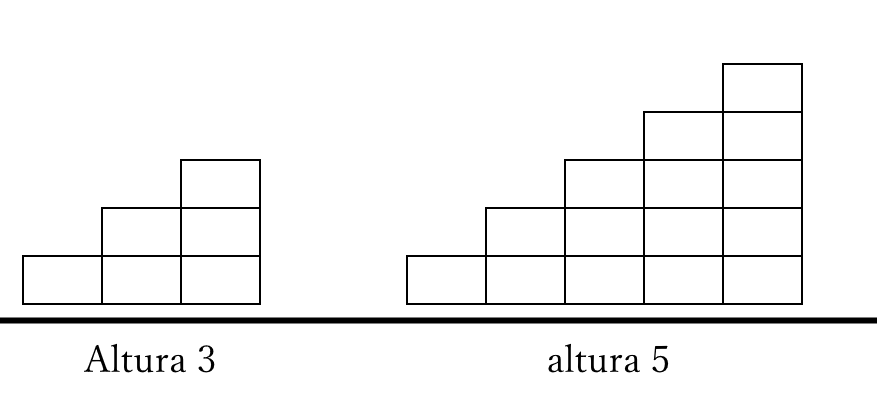
\includegraphics[scale=0.25]{escaleras}
\end{center}

El otro día, Fernando obtuvo \(K\) ladrillos, ahora se pregunta ¿Qué tan alto que puede construir una escalera? Dado \(K\), responde su pregunta.

\begin{plimits}
	\item \(1\leq K \leq 10^9\)
\end{plimits}

\subsubsection{Casos ejemplo}
\begin{casebox2}
	\scase{12}{4}
	\scase{8}{3}
	\scase{20}{5}
\end{casebox2}

Enlace: [TODO]

\section* {Búsqueda lineal con función de validación}
\addcontentsline{toc}{section}{Búsqueda lineal con función de validación}
\markboth{Búsqueda lineal con validación}{Búsqueda lineal con validación}

Hasta ahorita hemos visto problemas donde revisar si un candidato era la respuesta o no bastaba con un simple condicional, pero este no siempre es el caso.

Varías veces, para revisar si un valor es solución a nuestro problema, vamos a tener que necesitar un poco más de código e ideas. Veamos un problema de este estilo.

\section*{Ejemplo 1.3}
\addcontentsline{toc}{section}{Ejemplo 1.3}

\subsection*{Descripción}
Karel tiene \(N\) listones de distintas longitudes enteras. Karel quiere hacer pulseras con ellos, por lo que tomará cada uno de los listones y los cortará para que las pulseras usen segmentos del mismo tamaño.

A Karel le gustan los enteros, entonces la longitud de los segmentos también ha de serla. Además, Karel no quiere que sobre listón sin usar ¿Cuántos diferentes tamaños de segmento se pueden elegir?

\subsection*{Entrada}
Un entero \(N\), indicando la cantidad de listones
En la siguiente línea, \(N\) enteros indicando las longitudes de los listones. Llamemos \(A[i]\) a la longitud del listón \(i\).

\subsection*{Salida}
La cantidad de opciones para el tamaño de los segmentos

\subsection*{Caso ejemplo}
\begin{casebox3}
		\ecase{
			5 \\ 
			10 30 20}
			{3}
			{Las longitudes pueden ser 1, 2 y 5}
\end{casebox3}	
\subsection*{Límites}
\begin{plimits}
	\item \(1\leq N \leq 100\)
	\item \(1\leq A[i] \leq 5000\)
\end{plimits}

\subsection*{Código}
Encontremos con búsqueda lineal todos los tamaños de segmento que cumplen y contemos cuantos son.

Primero veamos que los tamaños de listón deben estar entre 1 y 5000. Más concreto, entre \(1\) y \(min (A[1],A[2],\cdots ,A[N])\). Esto es porque el tamaño del segmento debe ser entero, debe ser por lo menos 1 (ya que un segmento de tamaño 0 o menor no tiene sentido para este problema) y no puede ser más largo que el listón más corto.

Ya hemos visto como se ve una búsqueda lineal y la que usaremos en este caso sería:

\begin{lstlisting}
cin >> N;
for (int i=0; i< N; i++) {
	cin >> A[i];
}

int minA=A[0];
for (int i=1; i < N; i++) {
	minA=min(minA, A[i]); /* encuentra el liston mas
	pequeno. */
}
respuesta = 0;
for (int s =1; s <= minA; s++) {
	if (es s es un tamano de segmento valido) {
		respuesta++;
	}
}
cout << respuesta

\end{lstlisting}

Pero el reto ahora es el chequeo de “es s es un segmento de tamaño valido”.

Para esto necesitamos un poco más de trabajo. Veamos un solo listón. Si queremos cortarlo en segmentos de tamaño s sin que sobre, ¿qué tiene que cumplir s con relación al listón? Así es, que es, que s divida a la longitud del listón. Y podemos ver que s tiene que cumplir esto para todos los listones

Entonces, para ver que s sea una opción válida, hay que ver que s divida a todos los enteros en la lista de listones.

Para lograr esto, creemos una función booleana que se encargue de validar s.
\begin{lstlisting}
bool validar (int s) {
	bool respuesta = true;
	for (int i=0; i< N; i++) {
		if (A[i]%s!=0){
			respuesta = false;
			break;
		}
	}
	return respuesta;
}
\end{lstlisting}

Entonces con esta función obtenemos que el código de la búsqueda lineal ahora es:
\begin{lstlisting}
respuesta = 0;
for (int s =1; s <= minA; s++) {
	if (validar(s)) {
		respuesta++;
	}
}
cout << respuesta

\end{lstlisting}

Y con esto logramos completar el problema.

\subsection*{Complejidad}
La búsqueda lineal la hacemos sobre el valor de A, pero, además, por cada iteración de la búsqueda lineal, hacemos un ciclo que revisa la condición para que s sea contada.

Entonces, la complejidad nos queda como:   \(O(Busqueda\times Validar)=O(AN)\).

Como \(A\leq 5000\) y \(N\leq 100\). Nos queda que \(AN\leq 5\times 10^5\), lo cual corre en menos de un segundo.

\section*{Conclusión}
\addcontentsline{toc}{section}{Conclusión}
Habrá veces que en la búsqueda tengamos que hacer código para validar cada contacto que encontremos, y la complejidad de la validación se meterá como un factor a la complejidad de la búsqueda.  

Con esto obtenemos un algoritmo con complejidad \(O(Busqueda\times Validar)\).
\newpage
\section*{Problemas de práctica}
\addcontentsline{toc}{section}{Problemas de práctica}

\label{bicicleta}
\paragraph{Problema 1.6}  Karel ha comprado una bicicleta eléctrica con la que planea completar un recorrido. El recorrido se puede ver como \(N\) colinas en línea recta tal que la \(i\)-ésima colina tiene altura \(h_i\). Karel comienza en la colina hasta la izquierda y quiere terminar en la ultima colina de hasta la derecha.

Cuando Karel sube un metro gasta \(1\) unidad de energía, mientras que bajar un metro recupera \(1\) unidad de altura. Si Karel en algún momento necesita subir, pero su batería tiene 0 de energía, Karel se quedará atorado y no terminará el recorrido.

Por suerte al inicio hay una estación de recarga donde Karel puede recargar su bicicleta. Como nota, la batería tiene capacidad \(R\) y jamás podrá almacena más energía que \(R\).

Actualmente Karel tiene \(0\) de energía, Determina cuál es la menor cantidad de energía que es necesaria recargar al inicio para completar el recorrido. O determina si es imposible hacer el recorrido con la bicicleta de Karel.

\subsubsection*{Entrada}
La primera línea tiene dos enteros, el valor de \(N\) y \(R\).

En la siguiente línea vienen \(N\), enteros separados por espacios, siendo la altura de las colinas de izquierda a derecha. Recuerda que Karel comienza en la primera colina y quiera terminar en la última.
\subsubsection*{Salida}
Un entero, representando la menor cantidad de energía necesaria para completar el recorrido. Si Karel no puede completar el recorrido, imprime \(-1\).

\subsubsection*{Casos ejemplo}
\begin{casebox3}	
	\ecase{
		6 8\\
		4 6 3 5 7 
	}
	{3}
	{
		Karel inicia con 3 de energía, moverse de   \\
		la primera a la segunda colina le toma 2,  \\
		ahora tiene 1.\\
		Luego avanza y se recarga 3,\\
		ahora tiene 4.\\
		Después continua y se consume 2, ahora tiene 2. \\
		Vuelve a avanzar quedándose con 0 de energía. \\		
		Pero luego avanza y se recarga a 5. \\
		Finalmente avanza para termina con 5. \\
	}
	\ecase{
		5 6\\
		1 10 1 2 0
	}
	{-1}
	{}
	\hline
\end{casebox3}	

\subsubsection*{Límites}
\begin{plimits}
	\item \(2\leq N, R \leq 5000\)
	\item \(0\leq h_i\leq 5000\)
\end{plimits}

Fuente: OMIS online 2022.

Enlace: [TODO]

\problembreak

\paragraph{Problema 1.7} Un número capicúa es aquel que no cambia cuando se escribe al revés, por ejemplo \(34143\) y \(1221\) son capicúa, pero \(145\) no lo es porque \(145\neq 541\). Tampoco \(30\) es capicúa.

Determina cuantos números son capicúas entre \(L\) y \(R\).

\subsubsection*{Ejemplo}
Para \(L=1\) y \(R=50\) la respuesta es 13.

\subsubsection*{Límites}
\(1 \leq 1  \leq L \leq R \leq 10^5 \)

\problembreak

\paragraph{Problema 1.8} Dado \(L\) y \(R\), encuentra cuantos números primos\footnote{Un número es primo si y solo si tiene exactamente dos divisores positivos, el \(1\) y el mismo.} hay entre \(L\) y \(R\), incluyendo \(L\) y \(R\).
 

\subsubsection*{Entrada}
Dos enteros \(L\) y \(R\).
\subsubsection*{Salida}
La cantidad de números primos en el rango.
\subsubsection{Caso ejemplo}
\begin{casebox3}
	\ecase{1 7}{4}{Los primos contados son \(2,3,5\) y \(7\)}	
\end{casebox3}

\subsubsection*{Límites}
\begin{plimits}
	\item \(1\leq L \leq R \leq 10^5\)
\end{plimits}

Enlace: [TODO]


\chapter*{Búsqueda completa}
\addcontentsline{toc}{chapter}{Búsqueda completa}
\markboth{Búsqueda completa}{Búsqueda completa}

La búsqueda completa, también llamada fuerza bruta, es una técnica donde revisamos todos los posibles candidatos donde podría estar el o los valores que buscamos.

Esta búsqueda completa tiende a ser lenta, muchas veces incluso tiene complejidad exponencial y por esto, suele no ser la solución para los 100 puntos. Sin embargo, es muy útil conocerla ya que la fuerza bruta es fácil de pensar y siempre encuentra la respuesta si esta existe.

Ademas, la fuerza bruta suele resolvernos una o dos subtareas, dando un puntaje parcial. Esto es una forma de garantizar puntos en problema donde no se nos ocurra ideas mejores-

También hay muchos problemas que consisten en empezar de la fuerza bruta e ir mejorando de allí hasta que sea suficientemente buena.

No solo eso, además llega a ser útil para encontrar patrones y condiciones en las respuestas que no nos percatemos viendo la redacción, o para encontrar errores en un código que hayas hecho.


Las búsquedas completas suelen buscar la respuesta en:

\begin{plimits}
	\item Los elementos de un arreglo (búsqueda lineal)
	\item Los valores de un rango (búsqueda lineal)
	\item Las parejas
	\item Los ordenes o permutaciones
	\item Los subconjuntos
	\item Las cadenas de decisiones
\end{plimits}

Probablemente reconozcas la búsqueda lineal, y esto es resultado de que esta es la búsqueda completa más sencilla en la que revisamos de forma secuencial un rango donde se puede encontrar la respuesta. Pero búsqueda completa incluye más tipos de iteraciones que solo revisar los valores de un ciclo.

Veamos a continuación cada una de estos casos y aprendamos a trabajar con ellos.
\chapter*{Pares de elementos}
\addcontentsline{toc}{section}{Pares de elementos}
\markboth{Pares de elementos}{Pares de elementos}

En muchos problemas nos pedirán que encontremos o contemos la cantidad de pares que cumplan alguna condición, o nosotros convertiremos a un problema de este estilo. Para este tipo de problemas será útil conocer como hacer una búsqueda completa que revise todas las posibles parejas de elementos.

Como antes, veamos un problema que puede ser resuelto con esto.

\section*{Ejemplo 2.1.1}
\addcontentsline{toc}{subsection}{Ejemplo 2.1.1}

Fernando necesita \(K\) tornillos de la ferretería. Sin embargo, la vida no siempre es fácil y la ferretería no vende exactamente \(K\) tornillos.

Sin embargo, venden \(N\) cajas de tornillos cada una con \(C_i\) tornillos dentro. 

Como Fernando tiene una obsesión con no desperdiciar, él solo comprara las cajas de forma que traigan juntas exactamente \(K\) tornillos. Además, odia las bolsas de un solo uso que dan en la ferretería por lo que solo comprará dos cajas, una por cada mano.

Entonces, dado el tamaño de las cajas, determina si Fernando puede traer consigo exactamente \(K\) tornillos.

\subsection*{Entrada}
Dos enteros, \(N\) y \(K\), representando cuantas cajas hay y cuantos tornillos se requieren.

En la siguiente línea vendrán \(N\) enteros separados por espacios, indicando la cantidad de tornillos en cada caja.

\subsection*{Salida}
Deberás imprimir “SI” en caso de que Fernando pueda obtener K tornillos con sus reglas, o “NO” si es imposible.

\subsection*{Casos ejemplo}

\begin{casebox3}
	\ecase{
		4 6 \\
		3 1 8 5
	}
	{SI}
	{Usa las cajas con 1 y 5 tornillos.}
	\ecase{
		5 10\\
		3 1 8 5 12
	}
	{NO}
	{}
\end{casebox3}

\subsection*{Límites}
\begin{plimits}
	\item \(1\leq N \leq 1000\)
	\item \(1\leq K \leq 10^9\)
	\item \(1\leq C_i \leq 10^9\)
	\item \(C_i \neq K\)
\end{plimits}

Enlace: [TODO]

\section * {Solución}

Lo que nos pregunta el problema es: ¿Existe un par de cajas tal qué sumen \(K\)?

Para determinar si existe dicha pareja, lo que haremos será buscar entre todas las parejas de cajas aquella que sume \(K\). Es decir, buscaremos completamente todas las parejas posibles.

Para iterar por todas las parejas lo que haremos es primero definir una pareja como dos índices \((i,j)\), tal que \(0\leq i < j <N\).  Como queremos iterar por todos los posibles pares, primero iteraremos por todos los valores de \(i\). Y para cada \(i\), iteraremos por todas las \(j\) con las que se puede emparejar. El código se ve como:

\begin{lstlisting}
for (int i =0; i < N; i++) {
	for (int j=i+1; j< N; j++) {
		cout << i<<" "<<j<< "\n";/* imprimimos 
		cada par */ 
	}
}
\end{lstlisting}

Y ahora que sabemos iterar por todos los pares, lo utilizamos para revisar si existe un par que sume \(K\). 

\begin{lstlisting}
for (int i =0; i < N; i++) {
	for (int j=i+1; j< N; j++) {
		if (Caja[i]+Caja[j] == K) {
			cout << "SI";
			exit(0); /* Termina el programa, 
			encontramos la respuesta */
		}
	}
}
cout << "NO";
\end{lstlisting}

Entonces, son estos dos ciclos for nos permiten iterar por toda pareja de elementos en un arreglo. Esta es una herramienta bastante útil para resolver muchos problemas y subtareas.

\section * {Complejidad}
Bien, ahora hablemos de la complejidad de esta técnica. La complejidad es \(O(N^2)\). Esto es porque la cantidad de parejas con \(N\) elementos crece en\(O(N^2)\).

Pero incluso si no conocemos como crecen las parejas, podemos ver que este ciclo para \(i = 0\), itera por \(N-1\) valores de \(j\); para \(i=1\), iteramos por \(N-2\) valores de \(j\); para \(i=2\), iteramos por \(N-3\) valores de \(j\), y así sucesivamente. De forma que hacemos \((N-1)+(N-2)+\ldots+1+0\) iteraciones de \(j\). Entonces hacemos \(1+2+3+\ldots+(N-1)\) iteraciones.

Usando la formula se suma de gauss\footnote{Formula de gauss para sumar los primeros \(N\) naturales: \(1+2+3+\ldots+N=\frac{N(N+1)}{2}\)} obtenemos que:

\[1+2+3+\ldots+(N-1)=\frac{N(N-1)}{2}=\frac{N^2}{2}-\frac{N}{2}\]

Entonces, la complejidad queda como \(O(\frac{N^2}{2}-\frac{N}{2})=O(N^2)\)

Por lo tanto, iterar por todos los pares de un arreglo es una técnica de complejidad cuadrada, perfecta para límites hasta \(\sim{10^4}\).

\newpage
\section*{Problemas de práctica}
\addcontentsline{toc}{subsection}{Problemas de práctica}

\paragraph{Problema 2.1.1} Definimos una inversión como una parejas \((i,j)\) en un arreglo tal que \(1\leq i < j \leq N\) y también \(A_i > A_j\). Es decir, una pareja de números que estén al revés de como deberían estarlo en un orden de menor a mayor.

Dado un arreglo de \(N\) enteros, imprime cuantas inversiones hay en él.

\subsubsection*{Ejemplo}
\begin{casebox3}
	\ecase{
		4\\
		3 2 6 1
	}
	{4}
	{
		Las inversiones son: \\
		El 3 con el 2, \\
		el 3 con el 1,\\
		el 2 con el 1, \\
		y el 6 con el 1. 
	}	
\end{casebox3}
\subsubsection*{Límites}
\begin{plimits}
	\item \(1\leq N \leq 5000\)
	\item \(1\leq A_i \leq 10^9\)
\end{plimits}

Enlace: [TODO]

\problembreak

\paragraph{Problema 2.1.2} Fernando regreso el otro día a la tienda de tornillos, y esta vez quiere darle una puntuación en un sitio web de guías locales. Fernando juzga la calidad de la tienda en función de cuantas cantidades diferentes de tornillos él puede comprar.

Recordemos que la tienda vende \(N\) cajas de tornillos, cada una con \(C_i\) dentro. Recordemos que Fernando solo puede tomar una o dos cajas en una compra porque solo tiene dos manos.

Dado las cajas de tornillos, determina la calidad de la tienda.

\subsubsection{Ejemplo}
\begin{casebox3}
	\ecase{
		3\\
		1 3 4
	} 
	{5}
	{
	   Fer puede hacer compras de \\
	   1, 3, 4, 5 o 7 tornillos.
	}
\end{casebox3}

\subsubsection*{Límites}
\begin{plimits}
	\item \(1\leq N \leq 10^5\)
	\item \(1\leq A_i \leq 10^3\)
\end{plimits}

Enlace: [TODO]

\problembreak

\paragraph{Problema 2.1.3} La revista “algofashion” dijo esta semana que los números a la moda son aquellos que pueden ser representados como la suma de dos números pertenecientes a la secuencia de Fibonacci.

Recordemos que la secuencia de Fibonacci empieza con dos 1. Y luego cada número será resultado de la suma de los dos anteriores.
\[F_1=F_2=1\]
\[F_n=F_{n-1}+F_{n-2}\]

De forma que los primeros números de la secuencia son:
 \[1,1,2,3,5,8,13,21\ldots\]

Karel acaba de leer la revista y ahora quiere responder \(T\) preguntas, cada pregunta será del tipo: ¿El número \(x_i\) está de moda?

Como amigo, debes hacer un código que responda las dudas de Karel.

\subsubsection*{Entrada}
En la primera línea vendrá el valor de \(T\), cuantas preguntas tiene Karel.

En las siguientes \(T\) líneas vendrán las preguntas de Karel, una por línea. Cada pregunta consiste en un solo entero \(x_i\).

\subsubsection*{Salida}
Imprime \(T\) líneas, cada una siendo la respuesta a una pregunta de Karel. La línea \(i\) debe ser “SI” si \(x_i\) está a la moda y debe ser “NO” si no está a la moda. 

\subsubsection*{Caso ejemplo}	

\begin{casebox2}
	\scase{
		3\\
		5\\
		6\\
		10
	}
	{
		SI\\
		NO\\
		SI
	}
\end{casebox2}

\subsubsection*{Límites}

\begin{itemize}
	\setlength{\parskip}{1pt}	
	\item \(1\leq T \leq 100\)
	\item \(1\leq x_i \leq 10^{18}\)
\end{itemize}

Enlace: [TODO]

\problembreak

\paragraph{Problema 2.1.4} Tú tiene una constructora que busca comprar un terreno para construir un fraccionamiento.

Actualmente, el gobierno de Karelopolis permite que compres un terreno en la región para desarrollo. La región para desarrollo se ve como una cuadricula de \(N\) filas y \(M\) columnas. El terreno que compres debe ser rectangular y alineada a la cuadricula, es decir, no puedes comprar una celda de la cuadricula de forma incompleta.

Además, tu calculaste cuanto dinero obtendrías si compras cada celda, en concreto, la celda que esta en la fila \(i\) y columna \(j\) aportaría \(v_{ij}\) pesos. Como hay celdas con valor positivo y otras con valor negativo, te preguntas cual es el máximo valor que puedes obtener.

Por ejemplo, si la región para desarrollo se ve de la siguiente forma:

\begin{center}
		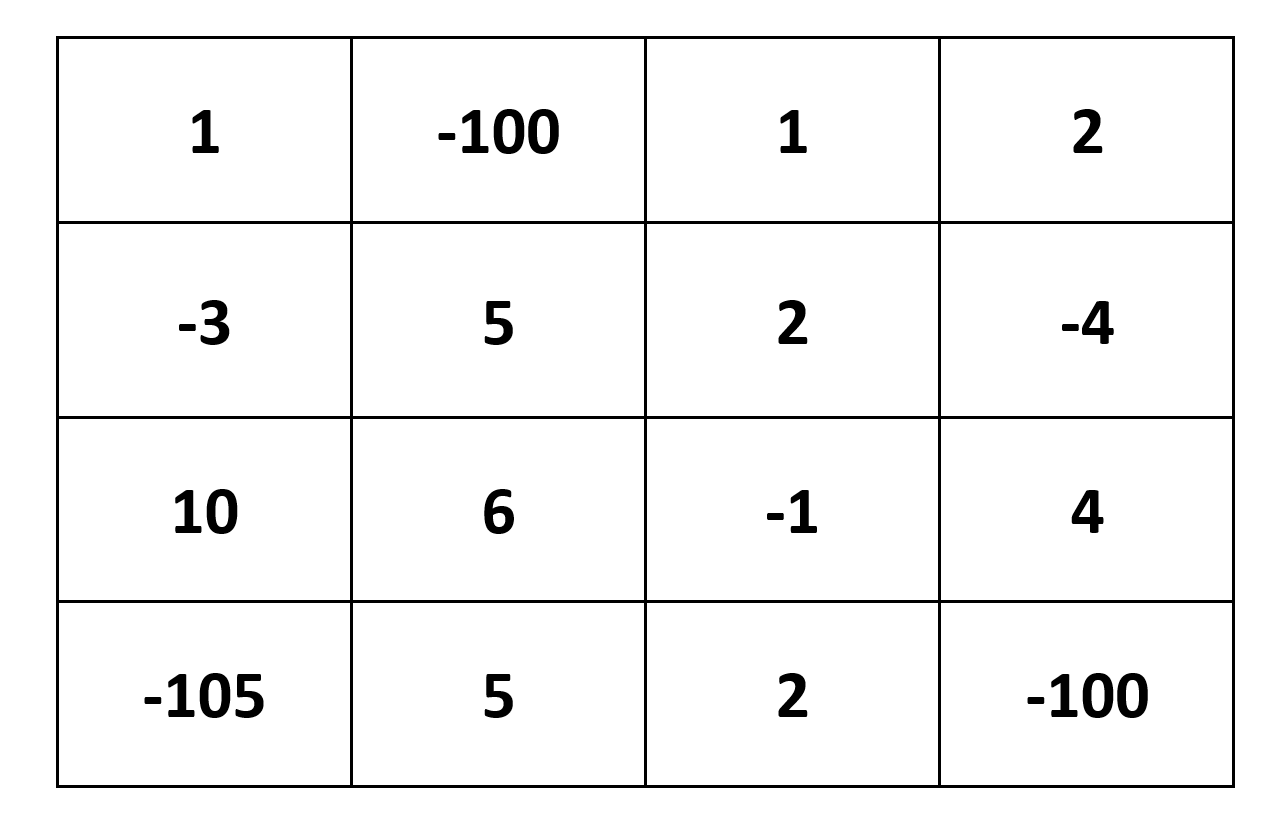
\includegraphics[scale=0.15]{terrenos}
\end{center}

Tu puedes obtener hasta 19 pesos comprando el terreno:

\begin{center}
	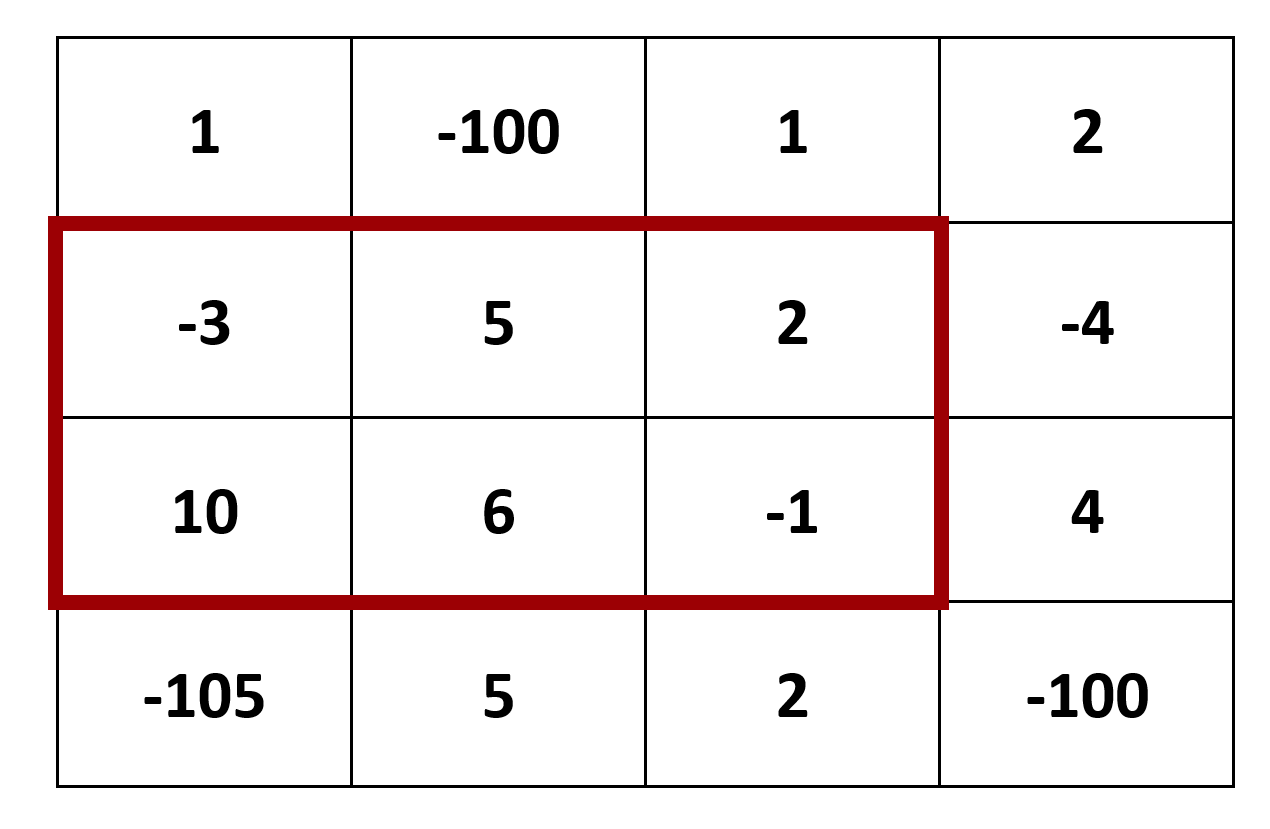
\includegraphics[scale=0.15]{terrenos2}
\end{center}


Encuentra el máximo valor posible si compras un terreno dada la región para desarrollo.

\subsubsection*{Entrada}

En la primera línea recibes \(N\) y \(M\).

En las siguientes \(N\) líneas recibirás \(M\) enteros representando los valores de \(v_{ij}\).

\subsubsection*{Salida}

Un entero que sea el mayor valor de un terreno.

\subsubsection*{Ejemplo}

\begin{casebox2}
	\scase{
		4 4\\
		1 -100 1 2\\
		-3 5 2 -4\\
		10 6 -1 4\\
		-105 5 2 -100
	}{19}
	\hline
\end{casebox2}

\subsubsection*{Límites}

\begin{plimits}
	\item \(1\leq N, M\leq 75 \)
	\item \(-10^9\leq v_{ij}\leq 10^9 \)
\end{plimits}

\subsubsection*{Subtareas}

\begin{plimits}
	\item (40 pts) \(1\leq N, M\leq 15 \)
	\item (60 pts) Sin consideraciones extra.
\end{plimits}

Enlace: [TODO]

\problembreak

\paragraph{Problema 2.1.5} Dado un arreglo \(A\) de \(N\) enteros. Determina si existe un par de elementos que su suma modulo \(P\) sea \(K\) .

\subsubsection*{Límites}
\begin{plimits}
	\item \(1\leq N,K,P\leq 10^5 \)
	\item \(1\leq A_i\leq 10^9 \)
\end{plimits}

\subsubsection*{Subtareas}
\begin{plimits}
	\item (25 puntos) \(1\leq N\leq 10^3 \)
	\item (50 puntos) \(1\leq K, P\leq 10^3 \)
	\item (25 puntos) Sin restricciones extra.
\end{plimits}

Codigo: [TODO]
\chapter*{Subconjuntos}
\addcontentsline{toc}{section}{Subconjuntos}
\markboth{Subconjuntos}{Subconjuntos}

Antes de aprender a buscar subconjuntos, comencemos definiendo que son. Una vez sepamos que son, veremos como resolver problemas con ellos.

\section*{Definición de conjuntos y subconjuntos}
\addcontentsline{toc}{subsection}{Definición}
Un conjunto no es nada mas que una colección de objetos. Por ejemplo, si alguien trae en su mochila un plátano, manzana y naranja, este puede decir que trae un conjunto de frutas compuesto por un plátano, manzana y naranja.

En matemáticas e informática, nosotros estamos trabajando todo el rato con los conjuntos. Ya sean el conjunto de datos de entrada, o los números enteros, tener noción de conjuntos es un requerimiento para el éxito en la olimpiada.

Veamos un poco de notación. Para escribir el conjunto A de números esta conformado por el 3, 5 y 9 escribimos lo siguiente:
\[A=\{3,5,9\}\]

TODO: CORREGIR ESTO
\newpage
\section*{Buscar subconjuntos}
\addcontentsline{toc}{subsection}{Buscar subconjuntos (ejemplo 2.2.1)}

Veamos como hacer para visitar todos los subconjuntos, lo cuál será necesario para problemas donde nos preguntan por ellos.

Para esto, primero aprendamos a resolver el problema que trata de mostrar los subconjuntos:

\subsection*{Ejemplo 2.2.1}

Karel tiene un conjunto formado por las primeras \(N\) letras del alfabeto. Ahora Karel que imprimas todos los subconjuntos, uno por cada línea. Puedes imprimirlos en cualquier orden.

Cada subconjunto es representado por las letras en el de la A a la Z. El subconjunto vacío será representado por un asterisco '*'.
\subsection*{Entrada}
Un entero \(N\), indicando cuantas letras hay en el conjunto.
\subsection*{Salida}
Todos los subconjuntos

\subsection*{Ejemplos}

\begin{casebox2}

	\scase{2}{
		AB\\
		A \\
		B\\
		*
	}
	\hline
\end{casebox2}

\begin{casebox2}
	\scase{3}
	{
		ABC \\
		AB \\
		AC\\
		A\\
		BC\\
		B\\
		C\\
		* \\
	}
\hline
\end{casebox2}

\subsection*{Límites}
\begin{plimits}
	\item \(1\leq N \leq 20 \)
\end{plimits}

\subsection*{Solución, iterar por subconjuntos}
Entonces, podemos resolver el problema si obtenemos todos los subconjuntos posibles. Para esto, haremos un algoritmo que construya todos los posibles subconjuntos.

Esto se puede hacer de dos formas principales, una iterativa y otra recursiva. Comencemos viendo la forma con recursión.

\subsection* {Subconjuntos usando recursión}

Digamos que \(S(conjunto)\) sean todos los subconjuntos del \(conjunto\). Por ejemplo:
\[S(\{A,B,C\})=\]
\[\{\{A,B,C\},\{A,B\},	\{A,C\},\{A\},\{B,C\},	\{B\},\{C\},	\emptyset\} \]

O usando la misma notación que la salida del problema (la que usaremos a partir de aquí):

\[S(ABC)=\{ABC, AB, AC, A, BC, B, C, * \}\]

Veamos un poco como se comporta S, por ejemplo para \(N = 4\), en total tenemos 16 subconjuntos los cuales podemos dividir en dos mitades con 8 cada una, los que tienen la A y los que no tienen la A.



\begin{center}
	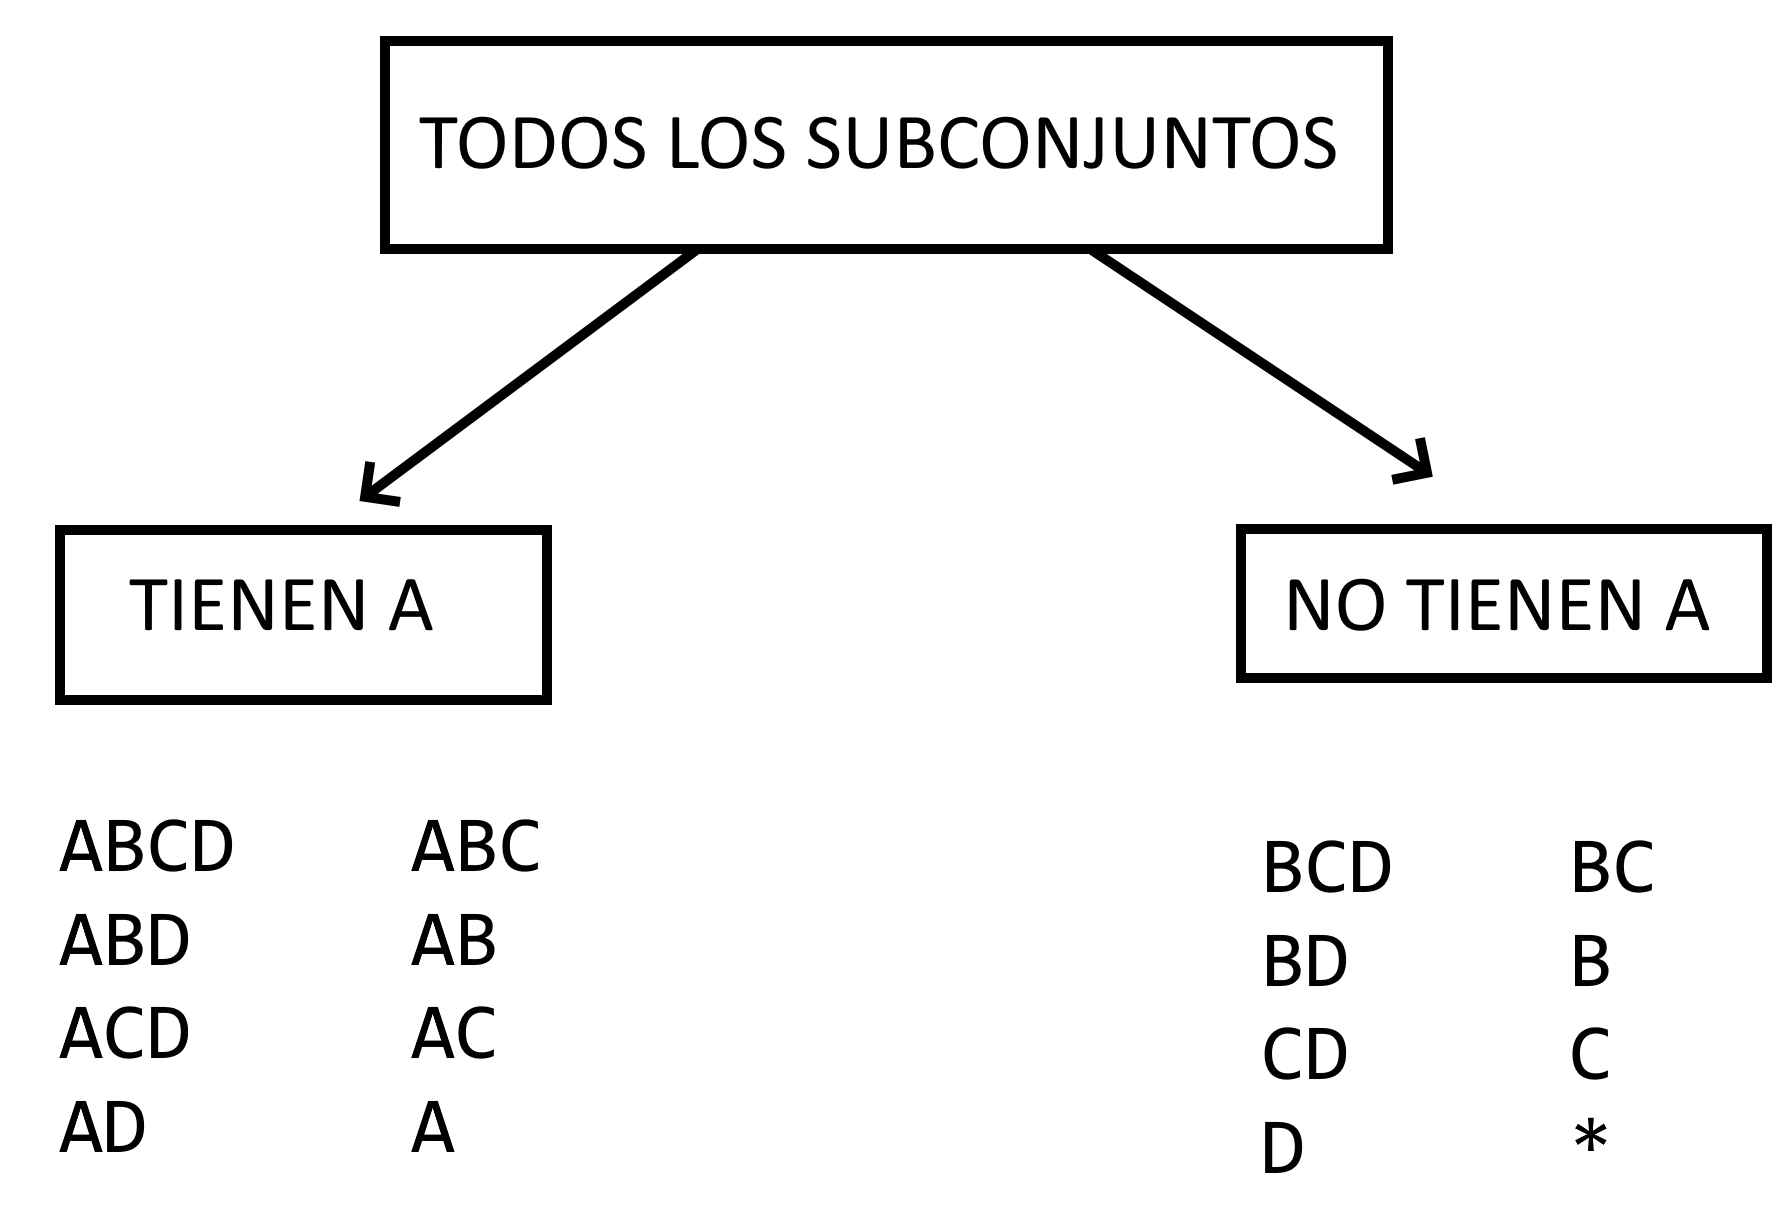
\includegraphics[scale=0.15]{subconjuntos1}
\end{center}

Ahora veamos que para los dos grupos, tenemos todos los 8 subconjuntos para \(BCD\), y lo único que los diferencia es si tienen \(A\) al inicio o no. Si supiéramos cuales son esos subconjuntos para las ultimas 3 letras, podríamos perfectamente construir \(S(ABCD)\), 

En concreto, podemos ver que \(S(ABCD) \) es igual a \(S(BCD)\) con \(A\) al inicio y \(S(BCD)\) sin nada extra. 

Si lo quieres ver en formula sería similar a \(S(ABCD)=A\rightarrow S(BCD) \cup S(BCD)\), donde \(A\rightarrow S(BCD)\) significa agregar \(A\) a todos los subconjuntos en \(S(BCD)\).

Y podemos hacer lo mismo, ver que \(S(BCD)\) es otra vez: los subconjuntos de \(CD\) con B y sin B.

Y de aquí obtenemos nuestro comportamiento recursivo.

Ahora que vemos la recursión, veamos una forma de implementar todo esto para resolver el problema.

Crearemos un metodo construyeSubconjuntos(int pos, int previo) que constuya los subconjuntos usando las letras desde pos hasta \(N-1\).
\pagebreak
\begin{lstlisting}
#include <iostream>
using namespace std;
int N;
char subconjunto[25];

// pos implica que letra estamos eligiendo si esta o no A=0, B=1, C=2, ...
// para N=6, pos = 2, es equivalente a  S(CDEF)
// previo indica cuantas letras se han agregaron a la construccion.
void construyeSubconjuntos(int pos, int previo) {
	if (pos == N) {
		//Ya no hay mas letras que decidir
		//imprime el subconjunto construido.
		if (previo==0) {
			cout <<"*\n";
		} else {
			cout << subconjunto<<"\n"; 
		}
		return;
	}
	//agrega la letra pos a la construccion
	subconjunto[previo]=pos+'A'; 
	construyeSubconjuntos(pos+1, previo+1); 
	
	// Quita la letra pos de la construccion
	subconjunto[previo]='\0'; 
	construyeSubconjuntos(pos+1, previo); 
	
}

int main () {
	cin >> N;
	construyeSubconjuntos(0,0);
	return 0;
}
\end{lstlisting}


De forma que el árbol de la recursión para construyeSubconjuntos(0,0) con \(N=2\) se ve:

 \begin{center}
	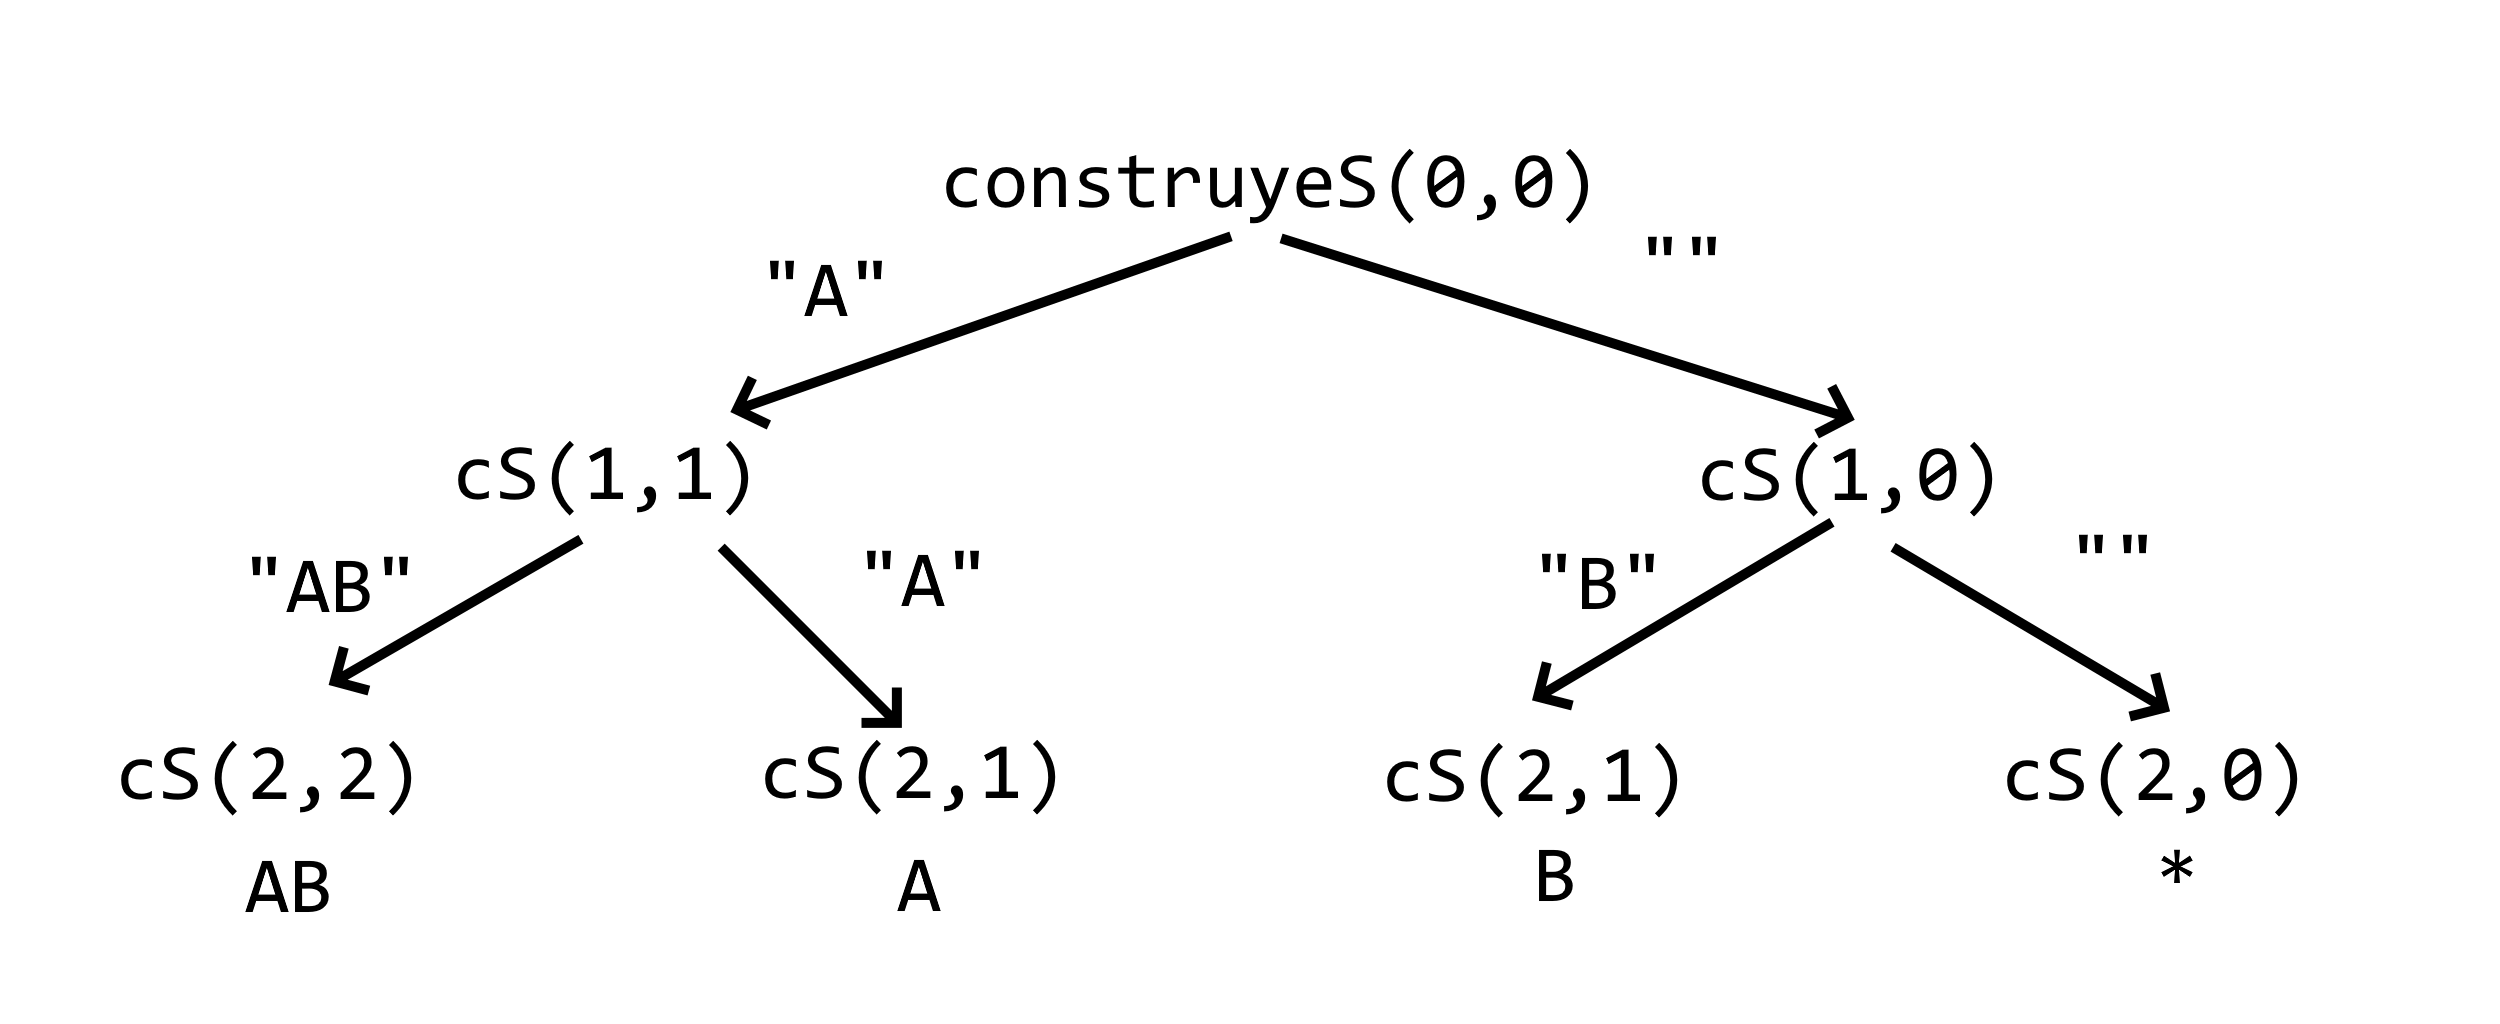
\includegraphics[scale=0.15]{AB}
\end{center} 

Un consejo para entender el código es simular la ejecución del programa paso a paso a mano en papel. Esto es útil cualquier otro algoritmo u técnica nueva.

\subsection*{Complejidad}
\addcontentsline{toc}{subsection}{Complejidad}
La complejidad de este código es igual a la cantidad de subconjuntos que se tienen con \(N\) elementos.

La primera forma de hacerlo es darnos cuenta que cada elemento tiene dos opciones, estar o no estar, por principio multiplicativo vemos que se multiplica por dos tantas veces como elementos tengamos. En total es \(2^N\) 

Esto es observable si recordamos el diagrama de las llamadas recursivas.

Vemos que por cada elemento, se divide en dos, duplicando la cantidad de llamadas en el proceso. En el primer nivel con pos=0, tenemos solo una llamada, con pos=1 tenemos dos, pos=3 obtenemos cuatro y así sucesivamente.

Por lo tanto, la complejidad es \(O(2^N)\), exponencial.

Una vez comprendido esto, pasemos a utilizar esto para resolver problemas.
\section*{Ejemplo 2.2.2}
\addcontentsline{toc}{subsection}{Ejemplo 2.2.2}

Fernando ha llegado a la ferretería con su objetivo frecuente de comprar \(K\) tornillos.  Sin embargo, la ferretería no siempre vende cajas con exactamente \(K\) tornillos dentro.

La ferretería tiene \(N\) cajas diferentes en venta, cada uno con \(C_i\) tornillos dentro.

Fernando quiere comprar unas cuantas cajas y obtener \textbf{exactamente} \(K\) tornillos. Por fortuna, esta vez trajo una bolsa y podrá comprar cuantas cajas le sea necesario.

Conociendo las cajas que venden en la Ferretería, determina si Fernando puede comprar los \(K\).

\subsection*{Entrada}
Dos enteros \(N\) y \(K\), la cantidad de cajas en la Ferretería y cuantos tornillos quiere Fernando.

En la siguiente línea vendrán la cantidad de tornillos en cada caja, los valores \(C_i\), separados por espacios.

\subsection*{Salida}
Debes imprimir "SI" en caso de que Fernando pueda comprar exactamente \(K\) tornillos. Caso contrario, imprime "NO".

\subsection*{Ejemplos}
\begin{casebox3}
	\ecase{
		5 10\\
		2 4 5 3 9	
	}
	{SI}
	{
		Compra la primera, tercera\\
		y cuarta caja.
	}
	\ecase{
		5 12\\
		4 5 2 11 3	
	}
	{NO}
	{}
\end{casebox3}
\subsection*{Límites}
\begin{plimits}
	\item \(1\leq N\leq 20 \)
	\item \(1\leq C_i\leq 10^9 \)
	\item \(1\leq K\leq 10^9 \)
\end{plimits}

\subsection*{Solución}

Como siempre, resumamos el problema en menos palabras. En corto, nos preguntan si existe un subconjunto de cajas tal que la suma de sus valores sea exactamente \(K\).

Y como es propio de todos los subtemas de búsqueda completa, veamos todas las posibles soluciones, es decir todos los subconjuntos, hasta que encontremos el que cumpla la condición o nos quedemos sin opciones.

Como ya vimos la forma de iterar por todos los subconjuntos en el ejemplo 3.1, utilicemos esas ideas para resolver este problema.

Lo que podemos hacer es ir construyendo todos los subconjuntos, esta vez en vez de representarlos como una cadena, lo representaremos como su suma. Esto en código se ve:
\newpage
\begin{lstlisting}
#include<iostream>
#include<stdlib.h>
using namespace std;
int Cajas[25];
int N;
long long K;
// Aqui, llevamos la suma del subconjunto construido
void buscaSubconjunto(int pos, long long suma) {
	if (pos==N) {
		if (suma == K) {
			/* Encontramos un subconjunto con suma K.
			Imprimmos SI y terminemos el programa */
			cout << "SI";
			exit(0);
		}
		return;
	}
	buscaSubconjunto(pos+1, suma+Cajas[pos]);//Incluyamos pos en el subconjunto
	buscaSubconjunto(pos+1, suma);//Excluyamos pos del subconjunto	
}

int main () {
	ios_base::sync_with_stdio(0); cin.tie(0);
	cin >> N >>K;
	for (int i=0; i < N; i++) {
		cin >> Cajas[i];
	}
	buscaSubconjunto(0,0);
	//Si llegamos aqui es porque nunca encontramos la respuesta.
	cout << "NO";
	return 0;
}
\end{lstlisting}

\newpage

\practiceproblemsection{2.2}

\problemtitle Warel se infiltro en una joyería con una mochila de capacidad \(W\).

En esta joyería hay \(N\) diamantes, cada uno tiene un valor de \(v_i\) y un peso de \(w_i\).

Warel puede robar cuantos diamantes quiera, pero el peso total de lo que se lleve no puede exceder a la capacidad de su mochila.

Determina la máxima cantidad de valor que Warel puede robar.

\subsubsection*{Entrada}
En la primera línea viene el valor de \(N\) y \(W\).

En la segunda línea vendrán los valores de los diamantes.

En la tercera y última línea vendrán los pesos de los diamantes.
\subsubsection*{Salida}
La máxima suma de valor que Warel puede robar.

\subsubsection*{Caso Ejemplo} 
\begin{casebox3}
	\ecase{
		5 6\\
		8 3 6 1 3\\
		5 1 3 2 6
	}
	{10}
	{
		Toma el segundo, tercer y cuarto diamante. \\
		Tendrás valor de \(10=3+6+1\) \\
		con peso \(6=1+3+2\)
	}
\end{casebox3}

\subsubsection*{Límites}

\begin{plimits}
	\item \(1\leq N\leq 20 \)
	\item \(1\leq W\leq 10^9 \)
	\item \(1\leq v_i, w_i\leq 10^9 \)
\end{plimits}

Enlace: [TODO]

\problembreak

\problemtitle Imprime todos los números binarios de \(N\) bits. 

Imprime los números de menor a mayor y agrega 0s a la izquierda para que todos los números tengan la cantidad correcta de bits.

\subsubsection*{Ejemplo}
\begin{casebox2}
	\scase{3}
	{
		000 \\
	  	001 \\
	  	010 \\
	  	011 \\
	  	100 \\
	  	101 \\
	  	110 \\
	  	111 \\
	}
	\hline
\end{casebox2}

\subsubsection*{Límites}
\begin{plimits}
	\item \(1\leq N \leq 20\)
\end{plimits}

\problembreak

\problemtitle  Un día encuentras una maquina que te permite invertir horizontalmente o verticalmente una matriz cuantas veces quieras. 

Invertir verticalmente significa intercambiar la primera y ultima fila, la segunda y penúltima fila, la tercera y antepenúltima fila, etc. Mientras que invertir horizontalmente es lo mismo, pero intercambias las columnas en vez de las filas.

Se te dan dos matrices \(A\) y \(B\), ambas de tamaño \(N\times M\). Determina si la maquina te permite convertir la matriz \(A\) en la matriz \(B\).

\subsubsection*{Entrada}
Los valores de \(N\) y \(M\).

Las siguientes \(N\) filas tendrán \(M\) enteros cada una. Siendo la matriz \(A\).

Y otra vez seguirán \(N\) filas con \(M\) enteros cada una. Los valores de la matriz \(B\). 

\subsubsection*{Salida}
Imprime "SI" en caso de que la matriz \(A\) pueda convertirse en la matriz \(B\).

\subsubsection*{Ejemplos}
\begin{casebox2}
	\scase{
		2 3\\
		1 2 3\\ 
		4 5 6\\
		6 5 4\\
		3 2 1
	}
	{SI}	
	\scase {
		2 2\\	
		1 2\\
		3 1\\
		2 3\\
		1 1
	} {NO}
\end{casebox2}

\subsubsection*{Límites}

\begin{plimits}
	\item \(1\leq N,M\leq 500 \)
	\item \(1\leq A_{ij}, B_{ij}\leq 10^9 \)
\end{plimits}

Enlace: [TODO]

\chapter*{Búsqueda binaria}
\markboth{Búsqueda binaria}{Búsqueda binaria}
\addcontentsline{toc}{chapter}{Búsqueda binaria}

Esta técnica es una de las más poderosas e importantes en la informática. Es una forma muy eficiente de hacer búsquedas que nos permite resolver problemas antes imposibles.

Utilizada en muchas aplicaciones, nos permite resolver problemas donde una búsqueda completa tardaría miles de millones de años en menos de un segundo. Y esta impresionante herramienta ahora será tuya.

La búsqueda binaria difiere de la completa al evitar revisar absolutamente todas las opciones del espacio de búsqueda. Si no, lo que hace es que en cada paso logra descartar la mitad del espacio de búsqueda al darse cuenta que la respuesta no está allí.

Porque en cada paso va descartando la mitad de las opciones, llega a una única opción (la respuesta si esta existe) en muy poco tiempo. Mientras que la búsqueda completa va eliminando opciones de una en una.

Comparemos un ejemplo de la búsqueda completa vs la binaria, si tuviéramos \(128\) candidatos. 

\begin{center}
	\begin{tabular}{|c|c|c|}
		\hline
		\multirow{2}{*}{\shortstack{Número\\ de pasos}} & \multicolumn{2}{c|}{Candidatos restantes} \\
		\cline{2-3}
		 & Completa & Binaria \\
		\hline
		0 & 128 & 128  \\		
		\hline
		1 & 127 & 64  \\		
		\hline
		2 & 126 & 32  \\
		\hline
		3 & 125 & 16  \\
		\hline
		4 & 124 & 8  \\
		\hline
		5 & 123 & 4  \\
		\hline
		6 & 122 & 2  \\
		\hline
		7 & 121 & 1  \\
		\hline
		8 & 120 &   \\	
		\multicolumn{3}{c}{
	\begin{LARGE}
	
		\(\cdots\)
		
	\end{LARGE} 
	}\\
		125 & 3 &  \\		
		\hline
		126 & 2 &  \\		
		\hline
		127 & 1 &  \\
		\hline
	\end{tabular}
\end{center}

Como vemos, búsqueda binaria pudo reducir los candidatos a solo uno con siete pasos, mientras que la búsqueda completa requirió de 127.

El motivo por el cuál la búsqueda binaria es tan efectiva, es que realiza \(\lceil log_2(candidatos) \rceil\) pasos \footnote{\(\lceil log_2(A) \rceil \) significa: techo del logaritmo base dos de A.\\ Recordemos que \(log_2(A)=x\) significa que \(2^x=A\).\\ Y el techo nos dice que tomemos el menor entero que sea mayor igual que el valor de adentro, por ejemplo:. \(\lceil 3.12 \rceil =4\)}. Esto es porque \(\lceil log_2 \rceil \) nos permite calcular cuantas veces podemos dividir un número entre dos hasta que sea 1.

Veamos un ejemplo que se puede resolver con búsqueda binaria.
\pagebreak
\section*{Ejemplo 3.1}
\addcontentsline{toc}{section}{Ejemplo 3.1}

Javier es un granjero y esta cansado de que sus animales siempre huyan de su granja, por lo que ha decidido poner una reja al rededor de todo el terreno.

Sin embargo, Javier no sabe cuantos metros de reja va a necesitar y te ha contratado para que tu le digas esto. 

Lo que él si sabe es que el tiene forma cuadrada con lados de longitud entera, además recuerda que este mide \(A\) metros cuadrados de área.

Ayuda a Javier para que sepa cuanta reja necesita.

\subsection*{Entrada}
Un entero \(A\), el tamaño del terreno en metros cuadrados.
\subsection*{Salida}
Un entero indicando cuantos metros de reja necesita para rodear todo el terreno. 

\subsection*{Ejemplos}
\begin{casebox2}
	\scase{36}{24}
	\scase{100}{40}
	\scase{1}{4}
\end{casebox2}

\subsection*{Límites}
\begin{plimits}
	\item \(1\leq A \leq 10^{18}\)
\end{plimits}
\subsection*{Subtareas}
\begin{plimits}
	\item (35 pts) \(1\leq A \leq 10^9\)
	\item (65 pts) Sin restricciones adicionales
\end{plimits}

\subsection*{Solución}
Como siempre, antes de leer la solución te invitamos a que intentes el problema.


En este problema nos piden de que dado el área de un cuadrado, imprimamos el perímetro. Por esto, recordemos las formulas del cuadrado.
\[Per\acute{i}metro=4\times Lado \]
\[\acute{A}rea=Lado\times Lado \]

Entonces, si encontramos el lado que nos de el área de entrada, podremos encontrar el perímetro.

Para este problema vamos a ver dos estrategias para resolverlo, la de búsqueda lineal y la binaria.

Comencemos con la que ya deberíamos estar familiarizada, usemos búsqueda lineal.

\subsubsection*{Búsqueda lineal}
Entonces, buscaremos el entero \(L\) de entre todos los posibles, que cumpla que \(A=4\times L\). Para esto, podremos ir probando del \(1\) en adelante hasta encontrar el que cumpla.

\begin{lstlisting}
	long long L=1;
	while (L*L != A) {
		L++;
	}
\end{lstlisting}

Esto itera por todos los enteros del \(1\) a la respuesta que es \(\sqrt{A}\). Por lo tanto, su complejidad es \(O(\sqrt{A})\). Lo cual corre para la subtarea de 35 puntos, pero no para el límite completo de \(10^{18}\).

\subsubsection*{Búsqueda binaria}
Ahora resolvamos el problema utilizando búsqueda binaria.

Definamos nuestro espacio de búsqueda, ¿cuáles valores puede ser \(L\)? y si lo pensamos puede ser desde \(1\) hasta \(10^9\). Porque \(10^9\times 10^9=10^{18}\) y de los límites sabemos que \(1\leq A\leq 10^{18}\).

Entonces queremos encontrar la respuesta que esta entre \(1\) y \(10^9\), hagamos una función que logre esto llamada buscar que reciba el rango de donde esta la respuesta.

\begin{lstlisting}
	//Encuentra L tal que L*L=A, sabiendo que a<=L<=b.
	long long buscar(long long a, long long b, long long A);
\end{lstlisting}

Ahora tenemos \(10^9\) candidatos donde encontrar la respuesta y queremos reducirlo a la mitad. 

Para esto podemos ver que sucede con \(5\times10^8\). 

Si resulta que \((5\times10^8)\times(5\times10^8) <A\), entonces sabemos que cualquier valor menor igual que \(5 \times 10^8\) no funcionará porque es demasiado pequeño. Por lo tanto la respuesta debe estar entre \(5\times 10^8 +1\) y \(10^9\) y los candidatos se redujeron a la mitad.

Pero si en vez sucede que \((5\times10^8)\times(5\times10^8) >=A\), entonces sabremos que cualquier valor más grande que \(5\times 10^8\) nos dará valores más grandes que \(A\) y por lo tanto la respuesta no estará allí. Ahora nuestros candidatos son los números entre \(1\) y \(5\times 10^8\), reduciendo los valores que podrían ser la respuesta a la mitad.

Y de hecho, si en general, la respuesta esta entre \(a\) y \(b\), nos convendrá preguntar por el punto medio \((a+b)/2\), que nos reducirá el espacio a la mitad.

Una vez que redujimos el rango de la búsqueda, tendremos que encontrar la respuesta en ese nuevo rango, y para esto podemos hacer recursión.

De forma que ahora tenemos:
\begin{lstlisting}
	long long buscar(long long a, long long b, long long A) {
		long long m =(a+b)/2;
		if (m*m < A) {
			return buscar(m+1, b, A);
		} else {
			return buscar(a, m, A);
		}
	} 
\end{lstlisting}

Ahora, lo que le falta a esa recursión es una condición de paro, saber cuando ya termino y encontramos la respuesta.

Podremos ver que habremos encontrado la respuesta cuando ya estemos seguros de cual es esta. Y esto sucede cuando nuestro rango solo incluye un valor, es decir, cuando \(a==b\) se cumpla.

\begin{lstlisting}
	long long buscar(long lonng a, long long b, long long A) {
		if (a==b)
			return a;
		long long m=(a+b)/2;
		if (m*m<A) {
			return buscar(m+1, b, A);
		} else {
			return buscar(a, m, A);
		}
	}
\end{lstlisting}

Y con esto, tenemos que \verb|L=buscar(1, 1000000000, A)|.

Ahora, la complejidad de esto es \(O(log(\sqrt{A}))\), lo cual corre perfectamente para \(10^{18}\).

\paragraph{Nota:} En este problemas también se pudo haber usado \verb|L=sqrt(A)| con la librería \verb|<math.h>| que calcula el valor rápidamente, pero se uso búsqueda binaria para ejemplificar.


\section*{Ejemplo 3.2}
\addcontentsline{toc}{section}{Ejemplo 3.2}
Se te da un arreglo \(A\) de \(N\) enteros diferentes. El arreglo estará en orden creciente, es decir, \(A[i] < A[i+1]\).

Deberás responder \(T\) preguntas:

Cada pregunta consistirá de un entero \(q_i\) y tu deberás imprimir el índice del valor \(q_i\) o \(-1\) si este valor no existe.
\subsection*{Entrada}
El enteros \(N\).

En la siguiente línea: \(N\) enteros separados, los valores del arreglo \(A\).

En la siguiente línea recibirás el entero \(T\).

En las siguientes \(T\) líneas recibirás los valores de cada pregunta.

\subsection*{Salida}
Imprime la respuesta cada pregunta en una línea en el mismo orden que el de lectura.

\subsection*{Ejemplo}
\begin{casebox2}
	\scase{
		7\\
		2 5 6 7 8 9 10\\
		5\\
		2\\
		6\\
		4\\
		10\\
		5\\
	}
	{
		0\\
		2\\
		-1\\
		6\\
		1		
	}
\end{casebox2}
\subsection*{Límites}
\begin{plimits}
	\item \(1\leq N,T \leq 10^5 \)
	\item \(1\leq A[i], q_i \leq 10^9 \)
\end{plimits}

Enlace: TODO

\subsection*{Solución}
Esta ocasión nos piden encontrar el indice de un valor en un arreglo ordenado. Ya hemos visto como hacerlo con búsqueda lineal:

\begin{lstlisting}
	int indice(int q) {
		for (int i =0; i < N;i++) 
			if (A[i]==q)
				return i;
		return -1;
	}
\end{lstlisting}

Sin embargo, esto no corre en tiempo ya que la complejidad es \(O(N)\) por pregunta, siendo en total \(O(TN)\) y como \(TN=10^{10}\), obtendremos TLE.

Pero veamos que podemos usar búsqueda binaria. ya que al preguntar por una posición de en medio y discernir si tenemos que buscar adelante o atrás.

\begin{lstlisting}
	int binaria(int a, int b, int q) {
		if (a>b)
			return -1;
		int m =(a+b)/2;
		if (A[m]==q)
			return m;
		if (A[m]<q) {
			return binaria(m+1, b, q);
		} else {
			return binaria(a, m-1, q);
		}		
	}
	int indice(int q) {
		return binaria(0, N-1, q);
	}
\end{lstlisting}

La nueva complejidad ahora es \(O(logN)\) por pregunta, en total\\ \(O(TlogN)\)

\section*{Dificultades}
\addcontentsline{toc}{section}{Dificultades}
Ya vimos que la búsqueda binaria tiene una ventaja enorme sobre la búsqueda lineal ya que resuelve el problema en un tiempo mucho menor.

Pero tristemente, no siempre es posible aplicar la búsqueda binaria. Hay veces en que las que no se puede descartar fácilmente la mitad de los candidatos.

Un caso donde puede suceder sería en el ejemplo anterior si el arreglo no estuviese ordenado. En ese caso no podríamos hacer el truco de solo revisar adelante si \(A[m]<q\) ya que no nos da suficiente información esa pregunta para eliminar todos los valores de \(0\) a \(m\).

Por supuesto, el problema anterior tiene corrección para que la búsqueda binaria siga funcionando y muchas veces esto es parte del problema, ¿cómo hago la binaria aquí? Pero hay otras veces que es imposible, o al menos, más allá de los conocimientos actuales.

En esos casos, no quedará de otra más que hacer búsqueda completa o usar una técnica diferente a búsqueda.

Otro ejemplo donde la búsqueda binaria no se puede utilizar es en encontrar el primer divisor que no sea 1 de un entero.
\newpage

\practiceproblemsection{3}

\problemtitle Fernando es el operador de montacargas en un almacén cuando le pidieron que sacara \(K\) piezas del inventario.

Sin embargo, las piezas están organizadas en una pila de \(N\) cajas. La caja \(i\) contiene \(C_i\) piezas.

Como funciona el montacargas, Fer puede agarrar las primeras \(R\) cajas de la pila y traerlas consigo.

Es decir, si \(C=[1,2,3,4]\) y \(R=2\), el montacargas se llevará las cajas \([1,2]\).

Como el montacargas gasta gasolina según cuantas cajas cargue y esta es muy cara, ayuda a Fer a determinar la mínima \(R\) para \(Q\) valores de \(K\).

\subsubsection*{Entrada}
Un entero \(N\) representando la cantidad de cajas.

En la siguiente línea habrá \(N\) enteros, los valores de \(C_1, C_2, \ldots, C_N\).

En la tercera línea estará el entero \(Q\), para cuantos valores debes descubrir \(R\).

En las siguientes \(Q\) líneas habrá un entero \(K\) que representa la cantidad de piezas deseada, suponiendo que siempre tenemos las mismas \(N\) cajas.

\subsubsection*{Salida}

Por cada una de las \(Q\) preguntas: imprime una línea con la mínima \(R\) para obtener \(K\) piezas, si no se puede imprime \(-1\).

\subsubsection*{Ejemplo}

\begin{casebox3}
	\ecase{
		3\\
		1 4 1\\
		3\\
		1\\
		3\\
		10
	}{
		1\\
		2\\
		-1
	}{
		Agarrando la caja No. 1 obtenemos 1 pieza\\ 
		\\
		Tomando la caja No. 1 y No. 2, tenemos 5\\ piezas, las cuales son mas que 3.\\
		\\
		No hay suficientes piezas para 10.
	}
	\ecase{
		5\\
		3 1 1 3 1\\
		1\\
		4
	}{
		2
	}{}
\end{casebox3}
\subsubsection*{Límites}
\begin{plimits}
	\item Para 50\%
	\begin{plimits}
		\item \(0< N \leq 10^2\)
		\item \(0< Q \leq 10^3\)
	\end{plimits}
	\item Para 100\%
	\begin{plimits}
		\item \(0< N \leq 10^5\)
		\item \(0< Q \leq 10^5\)
		\item \(0< C_i \leq 1000\)
		\item \(0\leq K \leq 10^9\)
	\end{plimits}
\end{plimits}

Enlace: \omegalink{Transporte-de-Cajas}



\problembreak

\problemtitle Sho colecciona juegos de dominó y quiere jugar.

Pero los dominós de Sho son un poco especiales, ya que son k-dominós. El dominó tradicional es del tipo 6-dominó, porque tiene números del \(0\) al \(6\), con un total de 28 fichas.

Entonces, un k-dominó tendrá números del \(0\) al \(k\). Con una ficha por cada par posible de números, incluyendo las mulas (mula es el mismo número emparejado consigo mismo).

Las fichas del 6-dominó son:

\begin{center}
		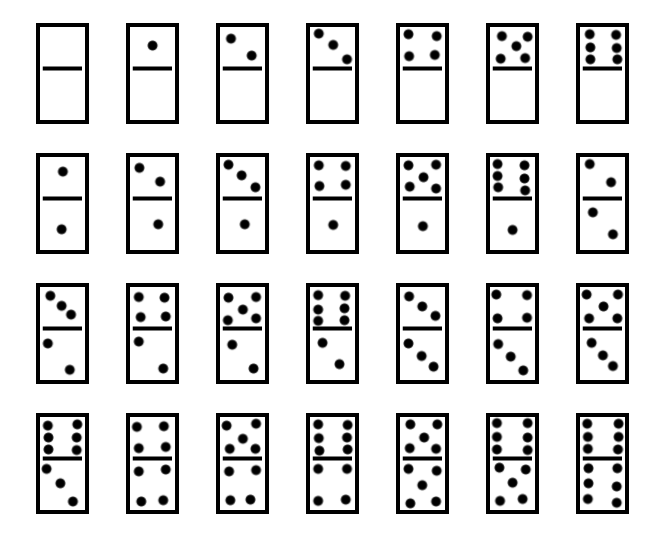
\includegraphics[scale=0.4]{domino6}
\end{center}

Y las del 2-domino son las siguientes seis:
\begin{center}
	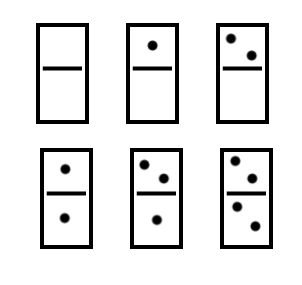
\includegraphics[scale=0.4]{domino2}
\end{center}

Sho quiere jugar con al menos \(N\) fichas, pero como después de jugar tiene que guardar, quiere usar el dominó con menor cantidad de fichas que tenga por lo menos \(N\) fichas. 

Dado \(N\), encuentra el valor de \(k\) para el k-dominó que le sirve a Sho.

\subsubsection*{Ejemplo}
\begin{casebox2}
	\scase{30}{6}
	\scase{6}{2}
	\scase{1000}{44}
\end{casebox2}

\subsubsection*{Límites}
\begin{plimits}
	\item \(1\leq N \leq 10^{18}\)
\end{plimits}

Enlace: TODO

\problembreak

\problemtitle Adivina el número que esta pensando OmegaUp.

Deberás implementar una función \verb|void adivina(long long a, long long b)| que descubra el número \(s\) que OmegaUp esta pensando. Se cumplirá que \(a\leq s\leq b\).

Para adivinar el número podrás llamar a la función \verb|long long pista(long long x)|.

Esta función regresará:
\begin{plimits}
	\item \verb|-1| si el número que piensa OmegaUp es menor que \(x\).
	\item \verb|0| si el número que piensa OmegaUp es \(x\).
	\item \verb|1| si el número que piensa OmegaUp es mayor que \(x\).
\end{plimits} 

La ultima llamada a pista debe ser con el número que OmegaUp esta pensando.

\subsubsection*{Límites}
\begin{plimits}
	\item \(-2^{61}\leq a,b \leq 2^{61}\)	
\end{plimits}
\subsubsection*{Evaluación}
Tu puntuación será en base a la cantidad de llamadas que hagas a la función \verb|long long pista(long long x)| de la siguiente manera:
\begin{plimits}
	\item 100\% si haces a lo más \(log(b-a+1)\)llamadas
	\item 50\% si haces a lo más \(2log(b-a+1)\)llamadas
	\item 0\% si haces más de \(2log(b-a+1)\)llamadas
\end{plimits}

Enlace: \omegalink{COMI-Adivina-el-numero}

NOTA: Este es un problema interactivo, si no conoces como trabajar con estos, ve la página: \pageref{interactivos}

\problembreak

\problemtitle A.R.C. Markland-N es un edificio alto con \(n\) pisos enumerados del \(1\) al \(n\). Entre cada dos pisos adyacentes existe una escalera que los conecta.

Es hora del almuerzo para nuestro sensei, Colin "ConneR" Neumann Jr, y él está planeando la ubicación donde disfrutar su comida.

La oficina de ConneR esta en el piso \(s\) del edificio. En cada piso (incluyendo \(s\)) hay un restaurante ofreciendo comida. Sin embargo, debido a renovaciones que están en proceso, \(k\) restaurantes se encuentran cerrados y por lo tanto, ConneR no puede disfrutar su almuerzo en ellos.

ConneR quiere llegar a un restaurante tan rápido como sea posible. ¿Cuál es el mínimo número de escaleras que debe usar para llegar al restaurante más cercano abierto?

\subsubsection*{Entrada}
En la primera línea habrá un entero \(t\) -- El número de casos pruebas. Luego vendrán las descripciones de cada uno de los \(t\) casos de prueba.

La primera línea de un caso de prueba tiene tres enteros \(n\), \(s\) y \(k\) -- Respectivamente, el número de pisos, el piso donde está ConneR y el número de restaurantes cerrados.

La segunda línea del caso de prueba tendrá \(k\) enteros distintos \(a_1, a_2 \ldots a_k\) -- Los números de piso con su restaurante cerrado.
\subsection*{Salida}

Por cada caso de prueba imprime una línea con la respuesta -- el mínimo número de escaleras que ConneR debe usar para llegar a un restaurante abierto.

\subsubsection*{Ejemplo}

\begin{casebox2}
	\scase{
		5\\
		5 2 3\\
		1 2 3\\
		4 3 3\\
		4 1 2\\
		10 2 6\\
		1 2 3 4 5 7\\
		2 1 1\\
		2\\
		100 76 8\\
		76 75 36 67 41 74 10 77		
	} {
		2\\
		0\\
		4\\
		0\\
		2
	}
\end{casebox2}
\subsubsection*{Límites}
\begin{plimits}
	\item\( 1 \leq t \leq 1000\)
	\item \(2\leq n \leq 10^9\)
	\item \(1\leq s \leq n\)
	\item \(1\leq k \leq min(n-1, 1000)\)
	\item Se garantiza que la suma de los valores de \(k\) no excederá \(1000\).
\end{plimits}

\codeforces

\codeforceslink{1293}{A}


\newpage
%------------------------------------------------------
\section*{Función de validación}
\addcontentsline{toc}{section}{Función de validación}
Igual que en búsqueda lineal podíamos agregar funciones más complicadas a la hora de buscar la respuesta, lo mismo sucede en búsqueda binaria. A veces requeriremos de más código que una simple comparación para saber en cual mitad esta la respuesta.

Veamos unos ejemplos.


\section*{Ejemplo 3.3}
\addcontentsline{toc}{section}{Ejemplo 3.4}
Karel ha comprado una bicicleta eléctrica con la que planea completar un recorrido. El recorrido se puede ver como \(N\) colinas en línea recta tal que la \(i\)-ésima colina tiene altura \(h_i\). Karel comienza en la colina hasta la izquierda y quiere terminar en la ultima colina de hasta la derecha.

Cuando Karel sube un metro gasta \(1\) unidad de energía, mientras que bajar un metro recupera \(1\) unidad de altura. Si Karel en algún momento necesita subir, pero su batería tiene 0 de energía, Karel se quedará atorado y no terminará el recorrido.

Por suerte al inicio hay una estación de recarga donde Karel puede recargar su bicicleta. Como nota, la batería tiene capacidad \(R\) y jamás podrá almacena más energía que \(R\).

Actualmente Karel tiene \(0\) de energía, Determina cuál es la menor cantidad de energía que es necesaria recargar al inicio para completar el recorrido. O determina si es imposible hacer el recorrido con la bicicleta de Karel.

\subsubsection*{Entrada}
La primera línea tiene dos enteros, el valor de \(N\) y \(R\).

En la siguiente línea vienen \(N\), enteros separados por espacios, siendo la altura de las colinas de izquierda a derecha. Recuerda que Karel comienza en la primera colina y quiera terminar en la última.
\subsubsection*{Salida}
Un entero, representando la menor cantidad de energía necesaria para completar el recorrido. Si Karel no puede completar el recorrido, imprime \(-1\).

\subsubsection*{Casos ejemplo}
\begin{casebox3}	
	\ecase{
		6 8\\
		4 6 3 5 7 
	}
	{3}
	{
		Karel inicia con 3 de energía, moverse de   \\
		la primera a la segunda colina le toma 2,  \\
		ahora tiene 1.\\
		Luego avanza y se recarga 3,\\
		ahora tiene 4.\\
		Después continua y se consume 2, ahora tiene 2. \\
		Vuelve a avanzar quedándose con 0 de energía. \\		
		Pero luego avanza y se recarga a 5. \\
		Finalmente avanza para termina con 5. \\
	}
	\ecase{
		5 6\\
		1 10 1 2 0
	}
	{-1}
	{}
	\hline
\end{casebox3}	

\subsubsection*{Límites}
\begin{plimits}
	\item \(2\leq N, R \leq 10^5\)
	\item \(0\leq h_i\leq 10^9\)
\end{plimits}

Fuente: OMIS online 2022.

Enlace: [TODO]

\section*{Solución}
Este problema 1.6 de búsqueda lineal con validación en la página \pageref{bicicleta}, si no sabes resolverlo con búsqueda lineal para los límites de allí, primero descubre esa solución.

Esta vez, los límites son más estrictos, de forma que la solución estándar con búsqueda lineal no funciona, pero veamos cual es porque nos será útil.
\\

La respuesta siempre estará entre \(0\)  y\(R\). La búsqueda lineal funciona de la siguiente manera.
\begin{lstlisting}
	int respuesta=-1;
	for (int e=0; e<=R; e++) {
		if (funciona(e)) {
			respuesta=e;
			break;
		}
	}
\end{lstlisting}

Y la función \verb|bool funciona(int e)| te regresa verdadero si Karel puede completar el recorrido comenzando con \(e\) de energía.

Esta función simplemente simula el recorrido para ver si Karel se atora en algún momento. Se ve de la siguiente forma:

\begin{lstlisting}
	bool funciona(int e) {
		for (int i = 1; i <N; i++){
			e-=A[i]-A[i-1];
			if (e > R) 
				e=R; //Limita la energia
			if (e < 0)
				return false;			
		}
		return true;
	}
\end{lstlisting}

La función \verb|funciona()| tiene una complejidad de \(O(N)\) y como es llamada en \(R\) valores, la complejidad total es \(O(RN)\).

Pero ahora veamos dos hechos importantes:
\begin{itemize}
	\item Si funciona(m) cumple, también lo hará cualquier valor mayor que \(m\).
	\item Si funciona(m) falla, también lo hará cualquier valor menor que \(m\).
\end{itemize}

Es decir, se ve de la siguiente forma:

TODO PONER IMAGEN AQUI

Esto hace que podamos hacer búsqueda binaria para encontrar el primer SI.

El código se verá como:

\begin{lstlisting}
	int a=0,b=R;
	while(a!=b) {
		int m=(a+b)/2;
		if (funciona(m)) {
			b=m;
		} else {
			a=m+1;
		}
	}
	int respuesta=-1;
	if (funciona(a))
		respuesta=a;
\end{lstlisting}

Ahora, recordemos que la complejidad de la búsqueda binaria es \(O(logR)\), pero en cada paso de la búsqueda estamos llamando a \verb|funciona()| que tiene complejidad \(O(N)\), por lo tanto, la complejidad total es \(O(NlogR)\).

\section*{Problemas de práctica}
\addcontentsline{toc}{section}{Problemas de práctica}

\problemtitle Barcos turísticos

El COMI ha preparado un paseo por barco para los olimpicos del OMI por el río \textit{algorrio}. 

El concurso está organizado por \(M\) delegaciones enumeradas del \(1\) al \(M\), cada una con \(a_i\) olímpicos.

Para este paseo se planean contratar \(K\) barcos en el que se subirán los olímpicos. Para que todo sea seguro, se debe poner un limite \(X\) de forma de que en un barco no pueda haber más de \(X\)  olímpicos abordo.

Para el abordaje, cada delegación se subira a un barco de forma que todos los olimpicos de la delegación esten en el mismo barco. Además, si en un barco esta la delegación \(x\) y la delegación \(y\) tal que \(x < y\), entonces también debe estar la delegación \(z\) en el mismo barco si se cumple que \(x < z < y\). En otras palabras, los barcos tendrán un rango consecutivos de delegaciones.

¿Cuál es la mínima \(X\) que permita que todos las delegaciones se suban a los barcos?

\subsubsection*{Entrada}
La primera línea tiene dos enteros \(M\) y \(K\) --la cantidad de delegaciones y barcos.

La segunda linea tendrá \(M\) enteros \(a_1, a_2, \ldots, a_M\) -- \(a_i\) es la cantidad e olimpicos en la delegación \(i\).

\subsubsection*{Salida}
Imprime un entero -- El menor valor de \(X\) que permita que todos los olímpicos se suban a algún barco.

\subsubsection*{Ejemplo}
\begin{casebox3}
	\ecase{
		5 3\\
		7 5 8 5 9
	}{13}{
		Los barcos serán\\
		1. La delegación 1 y 2\\
		2. La delegación 3 y 4\\
		3. La delegación 5	
	}
\end{casebox3}
\subsubsection*{Límites}
\begin{plimits}
	\item \(1\leq N, K \leq 10^5\)
	\item \(1\leq a_i \leq 10^9\)
\end{plimits}
TODO:
\omegalink{arg1}

\problembreak

\problemtitle Dado un arreglo \(A\) de \(N\) enteros, determina si existe un subcadena que sume \(K\).

Una subcadena es cualquier subarreglo de elementos continuos. Para el arreglo \([1, 2, 10, 5, 3]\), tenemos 15 subcadenas, algunas de estas son: \([1,2,10]\),
\([10,5]\), \([2,10,5]\), \([3]\).
\begin{plimits}
	\item \(1\leq N \leq 10^5\)
	\item \(1\leq A_i, K \leq 10^9\)
\end{plimits}


\newpage
\section*{Búsqueda en los reales}
\addcontentsline{toc}{section}{Búsqueda en los reales}

Hay veces en la que no estamos buscando un valor entero, si no en vez querremos encontrar un valor real a cierta precisión.

El problema dirá algo por el estilo de: imprime la respuesta con precisión de \(10^{-6}\), esto quiere decir que tu respuesta no debe estar alejada de la solución por más de \(10^{-6}\).

Para estos problemas debes cambiar la condición de paro de \(a==b\), por \(b-a < precision\). Aunque en realidad, recomiendo poner una precisión un poco más ajustada ya que no tiende a aumentar mucho el costo.

De forma que ahora la binaria se verá como:

\begin{lstlisting}
	double a =0, b=1e9;
	double epsilon = 1e-8;
	while(b-a>= epsilon) {
		double m = (a+b)/2;
		if (funciona(m)) {
			b=m;
		} else {
			a=m;
		}
	}
\end{lstlisting}

\section*{Ejemplo 3.5}
\addcontentsline{toc}{section}{Ejemplo 3.5}
Calcula la raíz cuadrada de un número A con precisión absoluta de \(10^{-4}\).
\subsection*{Ejemplo}
\begin{casebox2}
	\scase{10}{3.1622}
	\scase{16}{4.0000}
\end{casebox2}
\subsection*{Límites}
\begin{plimits}
	\item \(1\leq A \leq 10^9\)
\end{plimits}
\subsection*{Solución}
Usamos las mismas observaciones que usamos para el ejemplo 3.1, pero esta vez lo haremos con double y nos detenemos basados en una precisión.
\begin{lstlisting}
	double raiz(double A) {
		double a=0, b=A;
		while (b-a >= 1e-5) {
			double m=(a+b)/2;
			if (m*m < A) {
				a=m;
			} else {
				b=m;
			}
		}
		return a;
	}
\end{lstlisting}

\newpage
\section*{Problemas de practica}
\addcontentsline{toc}{section}{Problemas de práctica}
\problemtitle Fernando ha adquirido un gusto por las carreras de coches en la fórmula \(\pi\).

En este deporte, los coches recorren una pista recta que mide \(L\) metros de longitud. Además, dependiendo de resultados anteriores el coche \(i\) inicia con \(x_i\) metros de ventaja.

Como Fer es un aficionado muy dedicado, se ha percatado de que cada coche se moverá hacia la meta con una velocidad constante, en concreto, el carro \(i\) tendrá se moverá a \(v_i\) metros por segundo.

Fernando se pregunta, en que tiempo (medido en segundos) cruza el coche que termina en lugar \(K\).

\subsubsection*{Entrada}
Tres enteros \(N\), \(L\) y \(K\), la cantidad de coches en la carrera, la longitud de la pista y el lugar que te interesa.

En la segunda línea habrá \(N\) enteros, \(x_1, x_2, \ldots, x_n\), donde \(x_i\) es la posición inicial del coche \(i\).

En la tercera línea vendrán \(N\) enteros, \(v_1, v_2, \ldots, v_n\), donde \(v_i\) es la velocidad del coche \(i\).

\subsubsection*{Salida}
Un solo número, indicando el segundo en el cual pasa la meta el coche que termina en lugar \(K\). Con presición absoluta de menor o igual que \(10^{-6}\).

\subsubsection*{Ejemplos}
\begin{casebox2}
	\scase{
		4 10 2\\
		1 2 3 4\\
		3 3 1 10
	}  {
		2.666667
	}
\end{casebox2}
\subsubsection*{Límites}
\begin{plimits}
	\item \(1\leq N, L, K \leq 10^5\)
	\item \(1\leq v_i, \leq 10^3\)
	\item \(0 \leq x_i < L\)
\end{plimits}

\problembreak

\problemtitle Planetas: 

\omegalink{planetas} 

\problembreak

\problemtitle Foto

\omegalink{carretera}

\problembreak

\problemtitle La siguiente lección en preparatoria requiere que dos temas sean discutidos. El i-ésimo tema es interesante por \(a_i\) unidades para el profesor y \(b_i\) unidades para los estudiantes.

Un par te temas \(i\) y \(j\) (\(i<j\)) es llamado \textbf{bueno} si \(a_i+a_j > b_i+b_j\) (es decir, es más interesante para el profesor).

Tu tarea es encontrar el número de parejas de temas \textbf{buenas}.
\subsubsection*{Entrada}
Un entero \(n\), la cantidad de temas.

La segunda línea tiene \(n\) enteros: \(a_1,a_2,\ldots, a_n\), donde \(a_i\) es cuan interesante es el tema \(i\) para el profesor.

La tercera línea tiene \(n\) enteros: \(b_1,b_2,\ldots, b_n\), donde \(b_i\) es cuan interesante es el tema \(i\) para los estudiantes.

\subsubsection*{Salida}
Un entero, la cantidad de parejas buenas.

\subsubsection*{Ejemplo}
\begin{casebox2}
	\scase{
		5\\
		4 8 2 6 2\\
		4 5 4 1 3
	}{7}
	\scase{
		4\\
		1 3 2 4\\
		1 3 2 4
	}{0}
\end{casebox2}

\subsubsection*{Límites}
\begin{plimits}
	\item \(2\leq N\leq 2\cdot 10^5\)
	\item \(1\leq a_i, b_i\leq  10^9\)
\end{plimits}
\codeforces

\codeforceslink{1324}{D} 

\problembreak
\newpage
\section*{Binaria en C++}
\addcontentsline{toc}{section}{Binaria en C++}
En C++ hay algunas funciones ya programadas que pueden hacer búsqueda binaria por nosotros.

Principalmente reconocemos tres de estas, \verb|binary_search|, \verb|lower_bound| y \verb|upper_bound|.

Todas estas funciones requieren incluir \verb|<algorithm>|
\subsection*{Binary search}

Nos permite saber si un elemento concreto se encuentra o no en un arreglo ordenado.

A continuación se muestra un ejemplo de un arreglo con \(N\) elementos.
\begin{lstlisting}
	if (binary_search(arreglo, arreglo+N, elemento)) {
		cout << "Existe: "<<elemento<<" en el arreglo";	
	}	 else {
		cout << "No existe: "<<elemento<<" en el arreglo";	
	}
\end{lstlisting}

\subsection*{Lower bound}
Encuentra el primer elemento menor o igual que un valor en un arreglo ordenado. Si el elemento no existe, nos regresa un iterador al final.

Veamos como obtener el indice del elemento encontrado.

Con arreglos:
\begin{small}
\begin{lstlisting}
int posicion = 
	lower_bound(arreglo, arreglo+N, valor)-arreglo;
\end{lstlisting}
\end{small}

Con un vector queda como:

\begin{small}
\begin{lstlisting}
int posicion = 
	lower_bound(arr.begin(), arr.end(), valor)-arr.begin();
\end{lstlisting}
\end{small}

Si no hay elemento mayor o igual en el arreglo, obtenemos \verb|posicion=N|.

Lo que en realidad regresa \verb|lower_bound|, es un iterador, si te interesa más del tema, puedes leer sobre ellos en internet, para nosotros nos basta con saber la formula de arriba.

\subsection*{Upper bound}
Encuentra el primer elemento estrictamente mayor que un valor en un arreglo ordenado. 

Podemos usarlo como \verb|lower_bound|:

Con arreglos:

\begin{small}
\begin{lstlisting}
int posicion = 
	upper_bound(arreglo, arreglo+N, valor)-arreglo;
\end{lstlisting}
\end{small}

Con un vector queda como:

\begin{small}
\begin{lstlisting}
int posicion = 
	upper_bound(arr.begin(), arr.end(), valor)-arr.begin();
\end{lstlisting}
\end{small}

Obtendremos \verb|posicion = N| si no existe elemento estrictamente mayor que valor.



\chapter*{Búsqueda a profundidad}
\markboth{Búsqueda a profundidad (DFS)}{Búsqueda a profundidad (DFS)}
\addcontentsline{toc}{chapter}{Búsqueda a profundidad (DFS)}

\chapter*{Búsqueda en anchura}
\markboth{Búsqueda en anchura (BFS)}{Búsqueda en anchura (BFS)}
\addcontentsline{toc}{chapter}{Búsqueda en anchura (BFS)}

La BFS es similar a la DFS, en el sentido que explora todos los estados a los que se puede llegar a partir uno inicial.

Pero la diferencia es que esto los explora un orden diferente.

La DFS lo que hace es en un estado, explora totalmente lo que ofrezca una transición, y luego se regresa de esa exploración para ver la siguiente opción.

En cambio, la BFS lo que hace es llevar una lista de "estados por explorar" y procesarlos en orden. Para iniciar, revisamos todas las transiciones del estado inicial y los estados a los que nos lleven los agregamos en la lista.

\begin{center}
	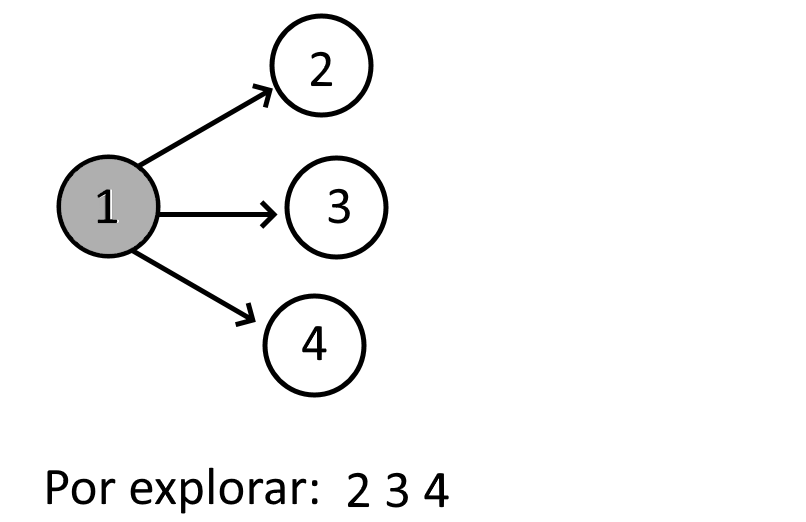
\includegraphics[scale=0.35]{bfs1}
\end{center}

Y luego para cada una de esos estados los exploramos también, es decir, expandimos las transiciones de esos estados y lo nuevo que encontremos lo ponemos en la lista de "estados por explorar". Importante: los visitamos en el orden que fueron agregados a la lista por explorar.

\begin{center}
	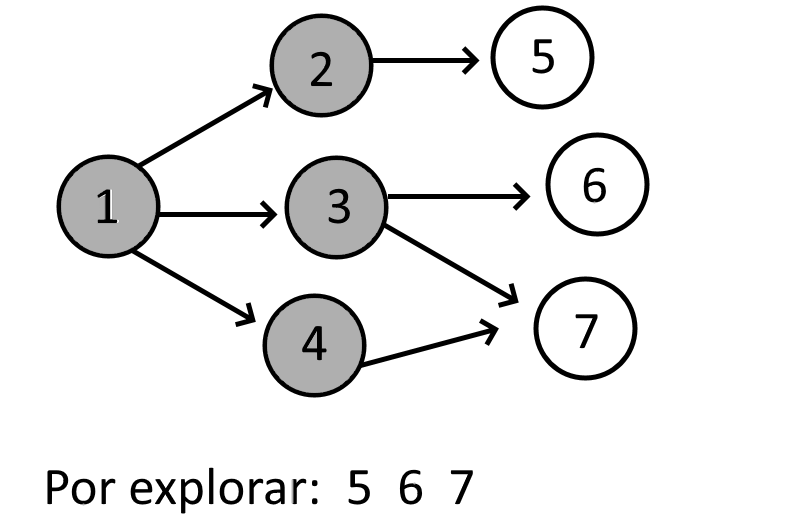
\includegraphics[scale=0.35]{bfs2}
\end{center}

De esta forma, comenzamos visitando todos los lugares alcanzables con una transición, luego dos transiciones, después tres, cuatro, cinco y  así sucesivamente.

Y precisamente, este orden en el que exploramos nos da una buena ventaja. A todo estado llegamos con la menor cantidad de transiciones posibles. Lo cual nos permite saber el mínimo número de transiciones necesarias para llegar e incluso lo podemos guardar en un arreglo o map para consultar después.

Para lograr este comportamiento, es importante ver que la lista por explorar se comporta de la siguiente forma: los estados son procesados en el mismo orden en el que entran, de forma que el primer estado en entrar a la lista es el primero en ser atendido. Este comportamiento es similar a la cola del cine, donde se atiende en el orden que llegas.

Para esto, podemos usar una estructura de datos de C++ llamada \verb|queue|, que significa cola en ingles. Si no sabes trabajar con ella, revisa el anexo en la página \pageref{queue}.

Entonces, una BFS lo que hace es:

Tener una cola de la lista por explorar llamada \verb|explorar|, un arreglo de booleanos \verb|visitado| para marcar los estados que ya han sido descubiertos por la BFS y agregaremos un arreglo de enteros \verb|no_transiciones| para guardar cuantas transiciones requerimos para llegar a cada estado.

Comenzamos agregando a la lista por explorar el estado inicial con un \verb|no_transiciones| de \(0\). Luego, mientras todavía allá estados por explorar, lo procesaremos. Lo sacaremos de la pila al ya ser explorado y agregaremos a \verb|explorar| todos los estados que no hayan sido visitados alcanzables desde el estado que estamos procesando.

En código:
\pagebreak
\begin{lstlisting}
bool visitado[];
int no_transiciones[];
void BFS(inicio) {
	queue<estados> explorar;
	cola.push(inicio);
	visitado[inicio]=true;
	no_transiciones[inicio]=0;
	while (explorar.empty()==false) {
		actual = explorar.front();
		cola.pop();
		if (actual es solucion) {
			registrar solucion actual;
			break; //opcional, si solo nos interesa una solucion
		}
		for (transiciones de actual) {
			if (!visitado[transicion]) {
				visitado[transicion]=true;
				no_transiciones[trancision]=
					no_transiciones[actual]+1;
				explorar.push(transicion);
			}
		}
	}
}
\end{lstlisting}
Como ya es de costumbre, veamos un ejemplo para entender esto.
\section*{Ejemplo 5.1}
\addcontentsline{toc}{section}{Ejemplo 5.1}
Javier tiene una calculadora un poco peculiar. Esta muestra un número \(x\) en pantalla y tiene dos botones.

\begin{plimits}
	\item El primer botón le suma \(a\) al valor de \(x\).
	\item El segundo botón le  suma \(\frac{x}{b}\) a \(x\), pero solo puede ser presionado cuando \(x\) sea un múltiplo de \(b\).
\end{plimits}

Ahora Javier se pregunta cuantas veces debe presionar un botón para que el valor \(x\) se convierta en \(y\).

\subsection*{Entrada}

La entrada constará de cuatro enteros: \(x\), \(y\), \(a\) y \(b\). El valor inicial de la calculadora, el valor deseado, y el valor de \(a\) y \(b\) para los botones.

\subsection*{Salida}
Imprime un entero que sea la cantidad de pulsaciones mínima para convertir \(x\) a \(y\). Si es imposible pasar de \(x\) a \(y\) imprime \(-1\).

\subsection*{Ejemplo}
\begin{casebox3}
	\ecase{	1 20 4 5}{6}
	{	Presiona el primer botón, ahora tienes 5.\\		
		Usa el segundo, ahora vale 6.\\
		Pulsa el primer botón, obtienes 10.\\
		Utiliza el segundo para tener 12.\\
		Usa el primer botón, obtén 16.\\
		Termina con el primero, llegamos a 20.
	}
	\ecase{	1 32 3 2}{-1}
	{	Es imposible obtener 32.
	}
\end{casebox3}

\subsection*{Límites}
\begin{plimits}
	\item \(1\leq x,y,a,b \leq 10^5\)
\end{plimits}

\section*{Solución}
Entonces, en este problema nos piden la mínima cantidad de operaciones para pasar de \(x\) al valor de \(y\).

Recordemos que la BFS es perfecta para esta situaciones, pues calcula la mínima cantidad de transiciones para pasar de un estado inicial a todos los demás, incluyendo \(y\).

Para esto haremos una BFS que use de estados el número de la calculadora y de transiciones los botones. Esta explorará todas las operaciones desde \(x\) hasta llegar a \(y\).

Esto se verá:

\pagebreak

\begin{lstlisting}
	bool visitado[100005];
	int no_transiciones[100005];
	int bfs(int x, int y, int a, int b) {
		queue<int> cola;
		cola.push(x);
		visitado[x]=true;
		no_transiciones[x]=0;		
		while (cola.empty()==false) {
			int actual=cola.front();
			cola.pop();
			if (actual==y) {
				return no_transiciones[y];
			}	
			//Primer boton
			int siguiente = actual+a;
			if (vistado[siguiente]==false){
				visitado[siguiente]=true;
				no_transiciones[siguiente]=
					no_transiciones[actual]+1;
				cola.push(siguiente);
			}
			//Segundo boton
			siguiente = actual+actual/b;
			if (actual%b == 0 && vistado[siguiente]==false){
				visitado[siguiente]=true;
				no_transiciones[siguiente]=
					no_transiciones[actual]+1;
				cola.push(siguiente);
			}
		}
		return -1;
	}
\end{lstlisting}



\section*{Complejidad}
\addcontentsline{toc}{section}{Complejidad}
La complejidad de una BFS es sencillamente de calcular. Veamos que cada estado es colocado una sola vez dentro de la cola y por lo tanto, explorado una sola vez.

Por lo tanto, cada transición también es visitada una única vez, cuando su estado correspondiente sea visitado.

Esto provoca que la complejidad de la BFS sea \(O(V+E)\), donde \(V\) es la cantidad de estados y \(E\) es el número de transiciones.

En el ejemplo 5.1, la cantidad de estados son a lo más \(y\) y a lo más tenemos dos transiciones por estado, por lo que la complejidad es \(O(V+E)=O(y+2y)=O(y)\).

\newpage

\practiceproblemsection{5}

\problemtitle Vasya encontró un dispositivo extraño. En el panel frontal hay: un botón rojo, un botón azul y una pantalla mostrando un entero positivo. 

Después de pulsar el botón rojo, el dispositivo multiplica por dos el número. Al pulsar el botón azul, el dispositivo le resta uno al número de la pantalla. 

Si en algún momento el número deja de ser positivo, el dispositivo se rompe. La pantalla puede mostrar números arbitrariamente grandes. Inicialmente se muestra el número \(n\).

Vasya quiere obtener el número \(m\) en la pantalla. ¿Cuál es la menor cantidad de pulsaciones que debe hacer para obtener este resultado?

\subsubsection*{Entrada}
La primera y única línea de la entrada tiene dos enteros distintos \(n\) y \(m\). 

\subsubsection*{Salida}
Imprime un solo número -- La mínima cantidad de veces que uno debe presionar los botones para obtener \(m\) del número \(n\).

\subsubsection*{Ejemplos}
\begin{casebox3}
	\ecase{4 6}{2}{Pulsa una vez el botón azul y luego el rojo.}
	\ecase{10 1}{9}{No necesitamos duplicar el número\\por lo que presionamos el azul nueve veces.}
\end{casebox3}

\subsubsection*{Límites}
\(1\leq n, m \leq 10^4\)

\codeforces  

\codeforceslink{520}{B}

\problembreak

\problemtitle Se te dan dos números enteros, \(n\) y \(x\). Tu puedes realizar múltiples operaciones al entero \(x\).

En cada operación que hagas consiste en: Elige un dígito \(y\) que este en la representación decimal de \(x\) al menos una vez, y remplazar \(x\) por \(x\cdot y\).

Quieres hacer que la longitud de la representación decimal de \(x\) (sin ceros a la izquierda) sea igual a \(n\). ¿Cuál es la menor cantidad de operaciones para lograr esto?

\subsubsection*{Entrada}
La única línea de la entrada contiene dos enteros \(n\) y \(x\).

\subsubsection*{Salida}
Imprime un entero -- El mínimo número de operaciones requeridas para hacer la longitud de la representación decimal de \(x\) (sin ceros a la izquierda) igual a \(n\), o \(-1\) si es imposible.

\begin{casebox3}
	\ecase{2 1}{-1}{}
	\ecase{3 2}{4}{
		1. multiplica \(x\) por \(2\), tal que \(x=2\cdot 2=4;\)\\
		2. multiplica \(x\) por \(4\), tal que \(x=4\cdot 4=16;\)\\
		3. multiplica \(x\) por \(6\), tal que \(x=16\cdot 6=96;\)\\
		4. multiplica \(x\) por \(9\), tal que \(x=96\cdot 9=864;\)\\
	}
	\ecase{13 42}{12}{}
\end{casebox3}
\subsection*{Límites}
\begin{plimits}
	\item \(2\leq n \leq 19\)
	\item \(1\leq x \leq 10^{n-1}\)
\end{plimits}
\codeforces

\codeforceslink{1681}{D}

\problembreak

\problemtitle Javier esta en un tablero de \(N\) filas y \(M\) columnas. En este tablero habrá unas celdas libres y unas celdas bloqueadas.

Él se encuentra en la casilla superior izquierda, la \((1, 1)\), y quiere llegar a la casilla \((f,c)\). La casilla donde Javier inicia siempre será libre.

Javier puede en cualquier momento, dar un paso y moverse a cualquiera de las cuatro casillas de arriba, abajo, izquierda o derecha. Siempre y cuando estas casillas existan y no estén bloqueadas. 

Determina la mínima cantidad de pasos para ir de \((1, 1)\) a \((f,c)\).

\subsubsection*{Entrada}
Dos enteros \(N\) y \(M\), el número de filas y el número de columnas del tablero.

En las siguientes \(N\) líneas recibirás \(M\) caracteres, siendo la descripción del tablero. '\#' simboliza una casilla bloqueada y '.' es una libre.

En la última línea tendrás dos enteros. \(f\) y \(c\), la fila y columna donde esta la celda a la que Javier quiere ir.

\subsubsection*{Salida}
Imprime un entero -- La mínima cantidad de pasos para ir de \((1, 1)\) a\((f, c)\). Si no se puede imprime \(-1\).

\subsubsection*{Ejemplo}

\begin{casebox3}
	\ecase{
		3 5\\
		\texttt{..\#.\#}\\
		\texttt{\#...\#}\\
		\texttt{..\#\#.}\\
		3 1
	} {		
		4
	}{
		\\
		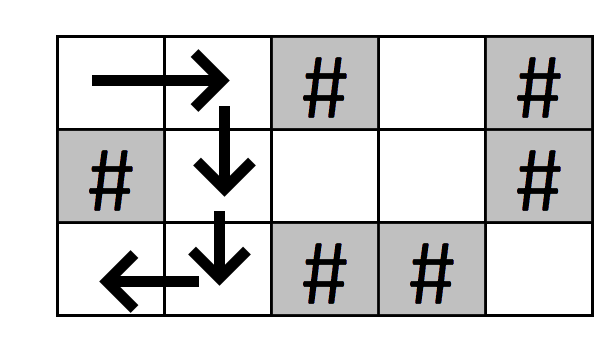
\includegraphics[scale=0.20]{caminoDFS1}
	}
	\ecase{	
		4 5\\
		\texttt{....\#}\\
		\texttt{\#...\#}\\
		\texttt{\#.\#\#.}\\
		\texttt{...\#.}\\
		3 5\\
	}{-1}{}
\end{casebox3}

\subsubsection*{Límites}
\begin{plimits}
	\item \(2\leq N, M\leq 1000\)
	\item \(1\leq f \leq N\)
	\item \(1\leq c \leq M\)
\end{plimits}

TODO \omegalink{}

\problembreak

\problemtitle Hay nueve relojes dispuestos en un arreglo de \(3 \times 3\) (véase la imagen), etiquetado con las las letras de la \(A\) a la \(I\). El objetivo d este problema  es regresar las manecillas de todos los relojes para que marquen las 12 en punto en el menor número de movimientos posibles.

\begin{center}
	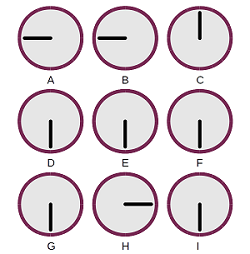
\includegraphics[scale=0.6]{relojes}
\end{center}

Hay nueve diferentes movimientos permitidos para modificar las manecillas de los relojes. Cada movimiento permitido es identificado por un número del 1 al 9. Un movimiento afecta únicamente a un determinado conjunto de relojes; cada reloj afectado mueve su manecilla 90° (grados) en sentido horario. A continuación se encuentra la descripción de los relojes afectados por los nueve movimientos:

\begin{center}
	\begin{footnotesize}
		\begin{tabular}{|ll|}
			\hline
			\thead{Movimiento} & \thead{Relojes afectados} \\
			\hline
			\makecell[c]{1} & \makecell[c]{ABDE} \\ \hline
			\makecell[c]{2} & \makecell[c]{ABC} \\   \hline
			\makecell[c]{3} & \makecell[c]{BCEF} \\  \hline
			\makecell[c]{4} & \makecell[c]{ADG} \\   \hline
			\makecell[c]{5} & \makecell[c]{BDEFH} \\  \hline
			\makecell[c]{6} & \makecell[c]{CFI} \\  \hline
			\makecell[c]{7} & \makecell[c]{DEGH} \\  \hline
			\makecell[c]{8} & \makecell[c]{GHI} \\  \hline
			\makecell[c]{9} & \makecell[c]{EFHI} \\  \hline
		\end{tabular}
	\end{footnotesize}
\end{center}

La siguiente figura muestra una posible solución para el caso presentado en la imagen de arriba, descrita por los números de movimiento 5, 8, 4 y 9. Nota que esta no es la única solución para el caso de ejemplo.


\begin{center}
	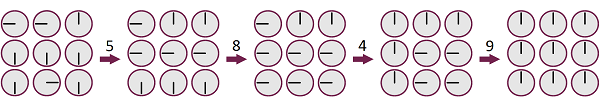
\includegraphics[scale=0.75]{relojes2}
\end{center}

\subsubsection*{Entrada}
res líneas con tres enteros cada una; cada entero representa la hora inicial de cada reloj, en el orden \(A, B, C, \ldots, H, I\). Los enteros tendrán un valor 3, 6, 9 o 12, representando la hora que marca un reloj.

\subsubsection*{Salida}
Imprime en salida estándar una sola línea con una lista de enteros separados por espacios: la secuencia de movimientos más corta que pone todos los relojes marcando las 12 en punto. En caso de que existan múltiples secuencias válidas con longitud mínima, cualquiera de ellas será aceptada.

\subsubsection*{Ejemplo}
\begin{casebox2}
	\scase{
		9 9 12\\
		6 6 6\\
		6 3 6
	}{5 8 4 9}
\end{casebox2}

Fuente: IOI 1994

\omegalink{relojes}






\chapter*{Problemas}
\addcontentsline{toc}{chapter}{Problemas}
\markboth{Problemas}{Problemas}
 \paragraph{P1}  
 
 \problembreak
 
 \paragraph{P2} Fuerza bruta
 
 \problembreak
 
 \paragraph{P3} Planetas: 
 
 
 \omegalink{planetas} 
 
  \problembreak
  
 \paragraph{P4} El COMI diseñó unos mapas futuristas. Los mapas futuristas son como los mapas de ahora, pero están impresos en una superficie transparente. Ellos tienen un archivo de varios mapas de la galaxia. Sebastian y Héctor se dieron cuenta de que existen varios mapas repetidos, por lo que desean eliminar cualquier repetición. Para esto, Sebastian toma un mapa, Héctor toma otro y ambos comparan los mapas para determinar si son iguales. Sin embargo, Héctor estaba distraído y algunos mapas se los pasaba en una posición diferente a la original. Ahora necesitan tu ayuda para comparar los dos mapas y saber si son iguales.
 
 Un mapa está representado por una matriz cuadrada de \verb|X|s y \verb|O|s. Dos mapas son iguales si ambos tienen el mismo carácter en la misma coordenada, para todas las coordenadas.
 
 Para validar que dos mapas son iguales, puedes aplicar cualquiera de las siguientes acciones cero o más veces sobre un mapa que quieras comparar con otro:
 \begin{plimits}
 	\item Rotarlo 90º.
 	\item Rotarlo 180º.
 	\item Rotarlo 270º.
 	\item Invertirlo horizontalmente.
 	\item Invertirlo verticalmente.
 \end{plimits}
 \begin{center}
 	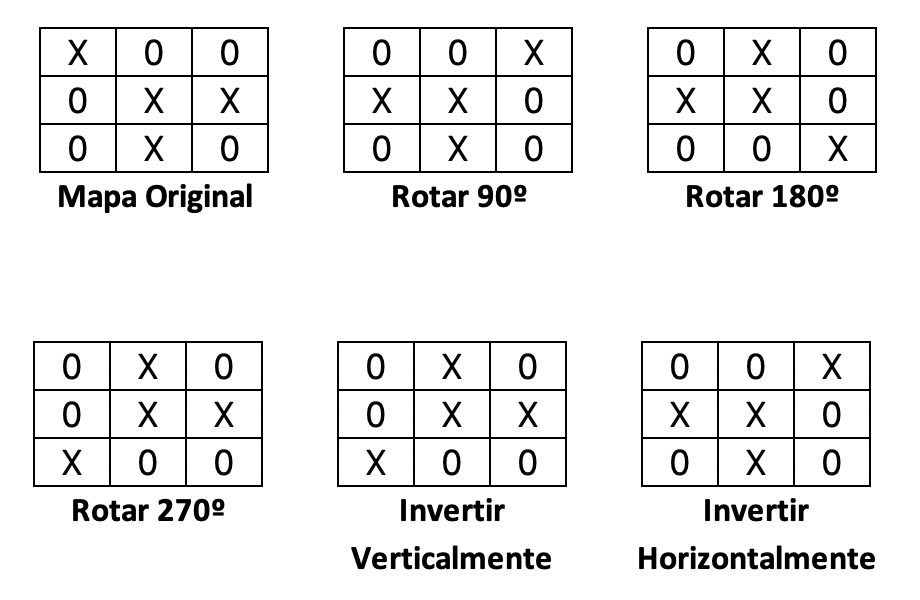
\includegraphics[scale=0.55]{mapasOMI2020}
 \end{center}
 
 \subsubsection*{Problema}
 Se te mostrará dos mapas y debes ayudarles a decir si son iguales o diferentes. Si son iguales, deberás escribir \verb|IGUALES|. Si son diferentes, deberás escribir \verb|DIFERENTES|.
 
 \subsubsection*{Entrada}
 En la primera línea \(N\), la longitud del lado de cada mapa. En las siguientes \(N\) líneas una cadena de \(N\) caracteres \verb|O| ó \verb|X| que representan el primer mapa. En las siguientes \(N\) líneas una cadena de \(N\) caracteres \verb|O| ó \verb|X| que representan el segundo mapa.
\subsubsection*{Salida}
Debes escribir \verb|IGUALES| si los mapas son iguales después de hacer todas las transformaciones necesarias o \verb|DIFERENTES| en caso contrario.

\subsubsection*{Ejemplo}
\begin{casebox3}
	\ecase{
		4\\
		XOOO\\
		XXOO\\
		OOOO\\
		XXXX\\
		XOOO\\
		XOOO\\
		XOXO\\
		XOXX
	}{IGUALES}{Si el segundo mapa lo giras 90º y además\\ lo inviertes verticalmente, obtienes \\la misma distribución que el primer mapa.}
	\ecase{
		2\\
		XX\\
		OO\\
		XO\\
		OX
	}{DIFERENTES}
	{No hay manera de transformar el segundo \\mapa para que se vea tal como el primero.}
	\ecase{
		4\\
		XOOO\\
		XXOO\\
		OOOO\\
		XXXX\\
		XOOO\\
		XXOO\\
		OOOO\\
		XXXX
	}{IGUALES}{
		En este caso los mapas ya son iguales,\\ sin necesidad de aplicar ninguna operación.		
	}
\end{casebox3}

\subsubsection*{Límites}
\(1 \leq N \leq 500\)
\subsubsection*{Subtareas}
\begin{plimits}
	\item (25 puntos)
	\begin{plimits}
		\item \(1\leq N \leq 10\)
		\item Se asegura que, en caso de que los mapas sean iguales, no es necesario aplicar ninguna acción.
	\end{plimits}
	\item (25 puntos)
	\begin{plimits}
		\item \(1\leq N \leq 50\)
		\item Se asegura que, en caso de que los mapas sean iguales, no es necesario aplicar ninguna rotación.
	\end{plimits}
	\item (25 puntos)
	\begin{plimits}
		\item \(1\leq N \leq 50\)
		\item Se asegura que, en caso de que los mapas sean iguales, no es necesario aplicar ninguna inversión vertical o inversión horizontal.
	\end{plimits}
	\item (25 puntos)
	\begin{plimits}
		\item \(1\leq N \leq 500\)
		\item Cualquier acción podría ser necesaria para validar que los mapas son iguales.
	\end{plimits}
\end{plimits}
 Fuente: \textbf{OMI 2020}
 
 \omegalink{OMI-2020-Mapas}
 
 
 \problembreak
 
 \paragraph{P5} DUMMY TODO
 
 
 \problembreak
 
 \paragraph{P6} DUMMY TODO


\problembreak
 
 \paragraph{P7} La siguiente lección en preparatoria requiere que dos temas sean discutidos. El i-ésimo tema es interesante por \(a_i\) unidades para el profesor y \(b_i\) unidades para los estudiantes.
 
 Un par te temas \(i\) y \(j\) (\(i<j\)) es llamado \textbf{bueno} si \(a_i+a_j > b_i+b_j\) (es decir, es más interesante para el profesor).
 
 Tu tarea es encontrar el número de parejas de temas \textbf{buenas}.
 \subsubsection*{Entrada}
 Un entero \(n\), la cantidad de temas.
 
 La segunda línea tiene \(n\) enteros: \(a_1,a_2,\ldots, a_n\), donde \(a_i\) es cuan interesante es el tema \(i\) para el profesor.
 
 La tercera línea tiene \(n\) enteros: \(b_1,b_2,\ldots, b_n\), donde \(b_i\) es cuan interesante es el tema \(i\) para los estudiantes.
 
 \subsubsection*{Salida}
 Un entero, la cantidad de parejas buenas.
 
 \subsubsection*{Ejemplo}
 \begin{casebox2}
 	\scase{
	 	5\\
	 	4 8 2 6 2\\
	 	4 5 4 1 3
 }{7}
	\scase{
		4\\
		1 3 2 4\\
		1 3 2 4
	}{0}
 \end{casebox2}

\subsubsection*{Límites}
\begin{plimits}
	\item \(2\leq N\leq 2\cdot 10^5\)
	\item \(1\leq a_i, b_i\leq  10^9\)
\end{plimits}
 \codeforces
 
 \codeforceslink{1324}{D} 
 

\problembreak

 \paragraph{P8} La leyenda dice que el tesoro de Moctezuma está enterrado en el Centro Histórico de la Ciudad de México. El Centro Histórico está representado como una cuadrícula de \(n\) filas y \(m\) columnas. Gracias a la tecnología de la nueva app iFind puedes desenterrarlo por fin.
 
 iFind es una app donde especificas una casilla \((i,j)\) de la cuadrícula y la app responde cuántos tesoros hay enterrados en el área del rectángulo que abarca de la fila \(1\) a la fila \(i\) y de la columna \(1\) a la columna \(j\).
 
 Una vez que sabes la casilla exacta donde hay un tesoro debes cavar en esa posición para desenterrarlo.
 
 Se asegura que cada casilla solo puede tener  o  tesoro y que no hay más de  tesoro en cada columna.
 
 \subsubsection*{Problema}
 Escribe un programa que dados \(n\) y \(m\), el alto y ancho de la cuadrícula y \(k\), el número total de tesoros enterrados, desentierre los \(k\) tesoros usando la menor cantidad posible de preguntas a la app.
 
 \subsubsection*{Interacción}
 No necesitas leer o escribir\footnote{Este es un problema interactivo, si no conoces como trabajar con estos, ve la página: \pageref{interactivos}}, debes implementar en tu código la función \verb|BuscaTesoros| y mandar llamar las funciones del evaluador \verb|Preguntar| y \verb|Cavar| para completar tu tarea.
 
 Internamente el evaluador llevará el registro de cuántos tesoros quedan. Tu programa no necesitará imprimir ni devolver nada: solo asegurarse de que hayas desenterrado los  tesoros usando la función Cavar.
 
\subsubsection*{Implementación}
\verb|void BuscaTesoros(int n, int m, int k);|

\textbf{Descripción:} El evaluador buscará en tu código esta función y la llamará con los parámetros \verb|n|, \verb|m| y \verb|k|. Tu implementación deberá utilizar las funciones \verb|Preguntar| y \verb|Cavar| para desenterrar todos los tesoros. En cada caso de prueba solo se llamará a esta función una vez.

\textbf{Parámetos}
\vspace{-\baselineskip}
\begin{plimits}
	\item \verb|n|: Filas de la cuadrícula.
	\item \verb|m|: Columnas de la cuadrícula.
	\item \verb|k|:  El número de tesoros enterrados.
\end{plimits}

TODO COMPLETAR

Fuente: \textbf{OMI 2018}
 
\omegalink{OMI2018-Tesoro}

\problembreak

\backmatter
% bibliography, glossary and index would go here.

\end{document}